% astra-rasti.tex — ASTRA RASTI Paper V5.0
% Original conversion from PDF text on 2026-04-04; enhanced to V2.0; revised to V2.1; V2.2 cross-domain
% Uses RASTI document class (rasti.cls)
%
% V5.0 revisions (2026-04-06):
%   - NEW: Stigmergic Swarm Intelligence subsection (Section 2.7) with full technical detail
%   - NEW: Figures 7-11 replaced with high-resolution dashboard screenshots (1920x1080)
%   - NEW: Self-Improvement and Adaptive Strategy subsection (Section 2.8)
%   - Updated results: 38 validated hypotheses, 397 total discoveries across 5 domains
%   - Abstract updated to mention stigmergy and swarm intelligence
%   - Added bibliography entries: Grasse1959, Gordon2010, Dorigo1996, Theraulaz1999
%   - Updated bibliography to references-v5
%
% V4.0 revisions (2026-04-05):
%   - Added new subsection: Operational Monitoring Dashboard (Section 2.7)
%   - Added Figure 7: 4-panel dashboard composite (Overview, Safety, Discoveries, Health)
%   - Added Figure 8: Safety dashboard detail (state space, anomaly detection, alignment)
%   - Added cross-references to dashboard from Discussion (safety, human-in-the-loop)
%   - Updated bibliography to references-v4
%
% V3.0 revisions (2026-04-05):
%   - Abstract trimmed from 321 to <250 words; removed inline citations and
%     parenthetical compilation details
%   - Tightened writing throughout: removed weasel words, reduced redundancy
%     between Discussion and earlier sections, strengthened topic sentences
%   - Tables 1 and 3: replaced \hline with booktabs (\toprule, \midrule,
%     \bottomrule); fixed Table 3 column spec (was 6, should be 5)
%   - Methods 2.1.1: removed "big questions" paragraph (kept in Discussion only)
%   - Methods 2.3: tightened 16-capability enumeration
%   - Methods 2.5: shortened positioning (detail in Discussion 9.4)
%   - TC2: merged duplicate AGN-fraction caveats into single paragraph
%   - Live Validation: fixed deployment count to six consistently throughout
%   - Discussion 9.1: reduced repetition of test-case results
%   - Discussion 9.4: trimmed overlap with Methods 2.5
%   - Discussion 9.5: trimmed overlap with Methods 2.1.1
%   - Conclusion: rewritten as narrative prose instead of bullet lists
%   - Removed dead/commented code; verified \citet vs \citep usage
%   - Changed \bibliography{references-v2} to \bibliography{references-v3}
%
% V2.3 revisions (2026-04-05):
%   - Sole author: Glenn J. White (Robin Dey removed from author block)
%   - Switched to RASTI document class (from mnras)
%   - Title: "Autonomous Scientific Discovery in Astrophysics"
%   - Acknowledgements: added OpenHub/Taurus platform credit
%   - Author Contributions: rewritten for sole author, OpenHub credited
%   - Dey2025 ref updated to STAN (vbrltech/STAN)
%   - WhiteDey2026 -> White2026 (sole-author bib key)
%   - All "the authors" -> "the author" (singular)
%
% V2.2 revisions (2026-04-04):
%   - Added cross-domain scientific validation (Section 8): economics (World Bank),
%     climate science (NASA GISS, NOAA Mauna Loa), epidemiology (World Bank Health),
%     cross-domain synthesis with FDR correction
%   - ~40 validated hypotheses across 5 scientific domains
%   - Phillips Curve failure highlighted as epistemic honesty
%   - New Discussion subsection "Cross-Domain Generalization"
%   - Updated abstract, introduction, scope, conclusion for cross-domain coverage
%   - Added acknowledgements for World Bank, NASA GISS, NOAA
%   - Added 8 bibliography entries
%   - Comprehensive Table 3 listing all ~40 hypotheses across 5 domains
%   - "Four Modes of Evidence" replacing "Three Modes"
%
% V2.1 revisions (2026-04-04):
%   - Corrected all quantitative claims to match actual pipeline outputs
%   - Added confounder analysis subsection
%   - Added 6 bibliography entries
%   - Strengthened Discussion; improved statistical reporting
%
% V2.0 enhancements:
%   - Strengthened introduction with ABT narrative structure
%   - Restored detailed TC3 sub-bullets
%   - Added Live System Validation section
%   - Enhanced abstract with quantitative highlights
%   - Updated codebase statistics (313,000+ lines, 621+ files)
%   - Added reproducibility note to Methods
%
\documentclass[usenatbib]{rasti}

% --- Packages ---
\usepackage{graphicx}
\usepackage{amsmath}
\usepackage{amssymb}
\usepackage{newtxtext,newtxmath}
\usepackage{hyperref}
\usepackage{xspace}
\usepackage{booktabs}

% --- Custom commands ---
\newcommand{\astra}{\textsc{Astra}\xspace}
\newcommand{\pc}{PC\xspace}
\newcommand{\fci}{FCI\xspace}

% ======================================================================
\title[ASTRA: Autonomous Scientific Discovery in Astrophysics]{ASTRA: Autonomous Scientific Discovery in Astrophysics}

\author[White]{
Glenn~J.~White$^{1,2}$\thanks{E-mail: glenn.white@open.ac.uk}\\
$^{1}$Department of Physics and Astronomy, The Open University, Milton Keynes MK7\,6AA, UK\\
$^{2}$RAL Space, STFC Rutherford Appleton Laboratory, Chilton, Didcot, Oxfordshire OX11\,0QX, UK
}
\date{Accepted XXX. Received YYY; in original form ZZZ}
\pubyear{2026}

\begin{document}
\maketitle

% ======================================================================
% ABSTRACT
% ======================================================================
\begin{abstract}
We present \astra (Autonomous System for Scientific Discovery in Astrophysics), an integrated framework that unifies numerical data analysis, causal reasoning, and physical validation within a single reproducible pipeline.
\astra chains dimensional analysis via the Buckingham $\pi$ theorem, structural causal models, Bayesian evidence computation, and multi-wavelength data fusion into coherent, physics-aware workflows.
A stigmergic swarm intelligence layer---inspired by ant colony foraging and calibrated using Gordon's biological parameters---coordinates hypothesis exploration through five specialized agents that deposit and follow digital pheromone trails, balancing exploration of novel domains against exploitation of productive research directions.
We validate the framework through six controlled astrophysical test cases, six live deployments recovering established physics (including Kepler's third law at $R^{2}=0.9982$), and cross-domain validation across economics, climate science, and epidemiology, collectively validating 38 hypotheses across five scientific domains.
\astra is a tool to assist scientists, not replace domain expertise.
Code and documentation: \url{https://github.com/Tilanthi/ASTRA}.
\end{abstract}

\begin{keywords}
methods: data analysis -- methods: statistical -- methods: general -- techniques: miscellaneous -- ISM: clouds -- stars: formation
\end{keywords}

% ======================================================================
\section{Introduction}
\label{sec:introduction}
% ======================================================================

Modern astronomical surveys generate petabytes of multi-wavelength data per year, and a rich ecosystem of computational tools---from classifiers to nested-sampling codes, from causal discovery algorithms \citep{Spirtes2000} to frontier large language models---gives astronomers unprecedented analytical power.
Yet these tools operate largely in isolation: astronomers must manually stitch together separate pipelines for data processing, statistical modelling, causal inference, and physical validation, creating opportunities for inconsistent treatment of uncertainties, missed physical constraints, and analyses that are difficult to reproduce.

\astra (Autonomous System for Scientific Discovery in Astrophysics) addresses this integration challenge.
Rather than replacing any single tool, \astra provides a unified framework that chains established algorithms into coherent, physics-aware analytical workflows.
The system combines:
\begin{itemize}
  \item Numerical data processing and statistical analysis
  \item Causal reasoning with structural causal models
  \item Physical validation through dimensional analysis and conservation laws
  \item Multi-wavelength data fusion with uncertainty propagation
  \item Hypothesis generation from pattern recognition
  \item Bayesian model selection with evidence computation
  \item Stigmergic swarm intelligence for autonomous exploration--exploitation balancing
\end{itemize}

This integrated approach ensures that physical validation, causal reasoning, and uncertainty quantification are applied consistently throughout multi-step analyses.
While individual components use established algorithms (\pc algorithm for causal discovery, bridge sampling for Bayesian evidence, the Buckingham $\pi$ theorem for dimensional analysis; \citealt{Buckingham1914}), their integration within a single framework enables analyses that would otherwise require manual combination of multiple separate tools.

In this paper, we focus on six examples demonstrating how this integrated approach can be applied to astrophysical inference problems:
\begin{enumerate}
  \item[(i)] \textbf{Scaling Relations Analysis} (Section~\ref{sec:tc1}): Dimensional analysis and physical validation of filament scaling relations
  \item[(ii)] \textbf{Multi-Wavelength Data Fusion} (Section~\ref{sec:tc2}): Probabilistic cross-matching with Bayesian uncertainty propagation
  \item[(iii)] \textbf{Pattern Recognition} (Section~\ref{sec:tc3}): Identification of established galaxy property relationships
  \item[(iv)] \textbf{Causal Inference} (Section~\ref{sec:tc4}): Structural causal model discovery in stellar data
  \item[(v)] \textbf{Bayesian Model Selection} (Section~\ref{sec:tc5}): Evidence-based model comparison with prior specification
  \item[(vi)] \textbf{Discovery-Mode Operation on Synthetic Data} (Section~\ref{sec:tc6}): Knowledge-isolated pattern discovery and causal inference on the star formation threshold problem
\end{enumerate}

The first five test cases use real observational data to validate \astra's ability to correctly recover known astrophysical results.
The sixth test case demonstrates discovery-mode operation beyond knowledge retrieval, under controlled conditions.
Using synthetic data with embedded causal structure (ground truth known to the author but not to \astra), it operates in ``knowledge isolation mode'' to discover patterns without being told what to look for, and generates testable predictions for future validation.

Section~\ref{sec:live} presents six live deployments on archival data that independently recover established physics.
To test whether \astra's analytical capabilities generalize beyond astrophysics, Section~\ref{sec:crossdomain} presents cross-domain validation across economics, climate science, and epidemiology using public data from the World Bank, NASA GISS, and NOAA.
Section~\ref{sec:discussion} discusses why these results demonstrate \astra's unique capabilities and clarifies \astra's role as a tool to assist rather than replace scientists, and Section~\ref{sec:conclusion} concludes.

% ======================================================================
\section{Methods: ASTRA System Architecture}
\label{sec:methods}
% ======================================================================

\subsection{Overview}
\label{sec:methods:overview}

\astra implements a modular architecture designed for astrophysical data analysis and inference.
The system integrates multiple specialized components through a coordinated framework, enabling complex multi-step analyses that combine data processing, physical reasoning, causal inference, and statistical validation.

\subsubsection{Scope and Limitations}
\label{sec:scope}

\textbf{What \astra Demonstrates:}
The six astrophysical test cases show that \astra can: discover physical laws from data with theoretical validation; fuse multi-wavelength observations with proper uncertainty handling; identify established astrophysical relationships through pattern recognition; distinguish causation from correlation; perform rigorous Bayesian model comparison; and operate in knowledge isolation mode to discover patterns and generate testable predictions beyond knowledge retrieval.
The cross-domain validation (Section~\ref{sec:crossdomain}) further demonstrates that these capabilities generalize to economics, climate science, and epidemiology, recovering approximately 42 validated hypotheses across five scientific domains.

\textbf{What \astra Does Not Claim:}
\astra is not presented as achieving artificial general intelligence or AGI-like performance.
The system operates within defined astrophysical domains using established algorithms (\pc algorithm, Bayesian inference, dimensional analysis via the Buckingham $\pi$ theorem, \fci causal discovery; \citealt{Zhang2008}) combined through an integrated architecture.
Results are validated against known physical theory and observational constraints.
The system does not claim general reasoning beyond its training domains or autonomous operation without human oversight; the live dashboard (Section~\ref{sec:methods:dashboard}) provides real-time safety monitoring and intervention controls.
The architecture supports natural language queries that trigger autonomous task completion, though this capability is not demonstrated in the present test cases.
A stigmergic swarm intelligence layer (Section~\ref{sec:methods:stigmergy}) coordinates autonomous exploration, while the live dashboard (Section~\ref{sec:methods:dashboard}) provides real-time monitoring and intervention controls.

\textbf{\astra's Role:}
\astra is a tool to assist the astronomer, not a replacement for domain expertise.
Its discovery architecture, used alongside an experienced scientist, provides capabilities in discovery and inference that go beyond those of straightforward AI or machine learning alone, as discussed in Section~\ref{sec:discussion:role}.

\textbf{Validation Scope:}
The first five test cases use real observational data to validate \astra's ability to correctly recover known astrophysical results.
The sixth test case demonstrates discovery capability on synthetic data with known ground truth, with testable predictions that require future observational validation.
The cross-domain validation (Section~\ref{sec:crossdomain}) extends the scope to five scientific domains using exclusively public data from established archives.
Generalization to additional domains or datasets requires further validation.

\subsection{Core Architectural Components}
\label{sec:methods:components}

\begin{enumerate}
  \item \textbf{Data Processing Pipeline:}
  \astra accepts heterogeneous astronomical data formats including catalogues (CSV, FITS), time-series data, images, and spectral data.
  The pipeline performs ingestion, validation, cleaning, and normalization while preserving measurement uncertainties and metadata.

  \item \textbf{Physics Engine:}
  A unified physics engine implements fundamental physical laws and constraints including conservation laws (mass, energy, momentum), dimensional analysis using the Buckingham $\pi$ theorem \citep{Buckingham1914}, equation solving and numerical simulation, and units consistency checking throughout calculations.
  This enables \astra to validate discoveries against first principles rather than treating correlations as sufficient explanations.

  \item \textbf{Causal Reasoning Module:}
  The causal reasoning module discovers and analyses causal structures using the \pc algorithm \citep{Spirtes2000} for learning directed acyclic graphs from observational data, the \fci algorithm \citep{Zhang2008} for causal discovery in the presence of latent confounders, conditional independence testing for continuous variables (Fisher's $Z$-test), V-structure detection for identifying colliders, do-calculus \citep{Pearl2009} for predicting effects of interventions, and domain-specific adaptations for astrophysical contexts.
  This module enables \astra to distinguish causal relationships from correlations, addressing a fundamental limitation of both traditional ML and LLM approaches.

  \item \textbf{Bayesian Inference Engine:}
  Rigorous model comparison and uncertainty quantification are performed through evidence computation via marginal likelihood estimation, Bayes factors for model comparison \citep{KassRaftery1995}, automatic complexity penalty (Occam's razor), posterior predictive checking, and Monte Carlo methods for uncertainty propagation.
  Model complexity is assessed using the Bayesian Information Criterion \citep[BIC;][]{Schwarz1978} as a rapid approximation where full evidence computation is unnecessary.

  \item \textbf{Domain Knowledge Systems:}
  Organized astrophysical knowledge through MORK ontology encoding taxonomic and causal relationships, knowledge graphs for semantic relationships, vector-based semantic memory for concept retrieval, and 75 specialized domain modules (ISM, star formation, exoplanets, etc.).

  \item \textbf{Multi-Module Orchestration:}
  Coordinates different analytical perspectives through specialized processing modules for different analysis types, a meta-cognitive layer for context-appropriate module selection, result synthesis and conflict resolution, and quality control and validation checks.
\end{enumerate}

\subsection{Unique Capabilities}
\label{sec:methods:capabilities}

\astra integrates sixteen distinct analytical capabilities organized into four groups:

\textbf{Causal and Statistical Analysis:}
(1)~\emph{Bias Detection}---identifies and quantifies observational biases from survey geometry and selection effects.
(2)~\emph{Scaling Relations Discovery}---discovers physical laws through dimensional analysis and functional form detection.
(3)~\emph{Causal Inference}---discovers causal structures using the \pc and \fci algorithms \citep{Spirtes2000,Zhang2008} and distinguishes physical laws from selection biases.
(4)~\emph{Model Selection}---compares competing theories using Bayesian evidence with proper complexity penalties.

\textbf{Data Integration and Analysis:}
(5)~\emph{Multi-Wavelength Fusion}---cross-matches sources across wavelengths with astrometric uncertainty propagation.
(6)~\emph{Uncertainty Quantification}---propagates measurement errors through first-order and Monte Carlo methods.
(7)~\emph{Temporal Reasoning}---detects periodic signals and forecasts time-series behaviour.
(8)~\emph{Instrument-Aware Analysis}---evaluates observational requirements across astronomical facilities.

\textbf{Knowledge Generation:}
(9)~\emph{Hypothesis Generation}---identifies patterns, detects anomalies, and generates testable hypotheses.
(10)~\emph{Analogical Reasoning}---discovers structural mappings between different astrophysical systems.
(11)~\emph{Counterfactual Analysis}---simulates physically-grounded scenarios to predict intervention effects.
(12)~\emph{Physical Model Discovery}---identifies functional forms and validates against theoretical predictions.

\textbf{Meta-Cognitive Capabilities:}
(13)~\emph{Meta-Cognitive Evaluation}---assesses data sufficiency, resolution limits, and observational constraints.
(14)~\emph{Anomaly Detection}---identifies unusual objects using ensemble methods.
(15)~\emph{Ensemble Prediction}---combines multiple models using Bayesian Model Averaging.
(16)~\emph{Physical Validation}---checks results against dimensional consistency, conservation laws, and established principles.

These capabilities are not independent modules but integrated components.
For example, discovering a scaling relation (capability~2) involves dimensional analysis (capability~12), physical validation (capability~16), and uncertainty quantification (capability~6).

\textbf{Capability Demonstrations in This Paper:}
Table~\ref{tab:capabilities} summarizes which of the 16~capabilities are demonstrated in each of the first five test cases.
Capabilities not demonstrated here (temporal reasoning, instrument-aware analysis, analogical reasoning, counterfactual analysis, ensemble prediction) are available in the system but demonstrated in extended test cases available in the GitHub repository.

\begin{table*}
  \caption{Capabilities demonstrated in each test case. \checkmark\ indicates the capability is explicitly demonstrated in that test case; -- indicates the capability is not applicable or not demonstrated in that test case.}
  \label{tab:capabilities}
  \centering
  \begin{tabular}{lccccc}
    \toprule
    Capability & Test~1 & Test~2 & Test~3 & Test~4 & Test~5 \\
               & (Scaling) & (Multi-$\lambda$) & (Pattern) & (Causal) & (Bayesian) \\
    \midrule
    Bias Detection              & --         & \checkmark & --         & \checkmark & --         \\
    Scaling Relations            & \checkmark & --         & \checkmark & --         & \checkmark \\
    Causal Inference             & --         & --         & --         & \checkmark & --         \\
    Model Selection              & --         & --         & --         & --         & \checkmark \\
    Multi-Wavelength Fusion      & --         & \checkmark & --         & --         & --         \\
    Uncertainty Quantification   & \checkmark & \checkmark & \checkmark & --         & \checkmark \\
    Temporal Reasoning           & --         & --         & --         & --         & --         \\
    Instrument-Aware Analysis    & --         & --         & --         & --         & --         \\
    Hypothesis Generation        & --         & --         & \checkmark & --         & --         \\
    Analogical Reasoning         & --         & --         & --         & --         & --         \\
    Counterfactual Analysis      & --         & --         & --         & --         & --         \\
    Physical Model Discovery     & \checkmark & --         & --         & --         & \checkmark \\
    Meta-Cognitive Evaluation    & \checkmark & \checkmark & \checkmark & \checkmark & \checkmark \\
    Anomaly Detection            & --         & --         & \checkmark & --         & --         \\
    Ensemble Prediction          & --         & --         & --         & --         & --         \\
    Physical Validation          & \checkmark & \checkmark & \checkmark & \checkmark & \checkmark \\
    \bottomrule
  \end{tabular}
\end{table*}

\subsection{Workflow for Scientific Analysis}
\label{sec:methods:workflow}

\astra's analysis workflow follows this general pattern:
\textbf{Input:}~Scientific query or observational data;
\textbf{Module Selection:}~Meta-cognitive layer selects appropriate analysis modules based on query type and data characteristics;
\textbf{Analysis Execution:}~Selected modules perform their specialized analyses including statistical and ML algorithms for pattern detection, causal discovery for identifying relationships, physics engine for theoretical validation, and Bayesian inference for model comparison;
\textbf{Integration:}~Results synthesized from multiple modules, resolving conflicts and identifying consensus conclusions;
\textbf{Validation:}~Results checked against physical constraints (dimensional consistency, conservation laws), statistical significance ($p$-values, confidence intervals), observational constraints (resolution limits, selection effects), and domain knowledge (established theories, previous results);
\textbf{Output:}~Integrated results with confidence assessments, uncertainty quantification, and physical interpretation.

\subsection{Implementation and Availability}
\label{sec:methods:implementation}

\astra is implemented in Python with approximately 313\,000 lines of code across 621~files.
The system uses established scientific Python libraries (NumPy, SciPy, Pandas, scikit-learn) combined with specialized implementations for causal discovery (\textsc{causal-learn}, \textsc{dowhy}), Bayesian inference (\textsc{dynesty} for nested sampling), and physics simulation (\textsc{astropy} for astronomical constants and coordinate transformations).

\textbf{Reproducibility:}
\astra requires Python~3.10 or later.
Key dependencies and their versions are specified in the repository's \texttt{requirements.txt}; the principal packages are \textsc{causal-learn} (causal discovery), \textsc{dynesty} (nested sampling), \textsc{astropy} (astronomical utilities), and \textsc{scikit-learn} (machine learning).
All results in this paper can be reproduced from the provided Jupyter notebooks using these dependencies.

The complete system is publicly available at: \url{https://github.com/Tilanthi/ASTRA} \citep{White2026}.
This repository includes: complete source code and installation instructions; system architecture documentation with detailed design diagrams; API documentation and user manual; extended validation with 15~comprehensive test cases; example notebooks and tutorials; and reproducible code for all results presented in this paper.
The first five test cases can be reproduced using the following Jupyter notebooks:
\texttt{test02\_scaling\_relations.ipynb} (Section~\ref{sec:tc1}),
\texttt{test04\_multiwavelength\_fusion.ipynb} (Section~\ref{sec:tc2}),
\texttt{test05\_hypothesis\_generation.ipynb} (Section~\ref{sec:tc3}),
\texttt{test11\_causal\_inference.ipynb} (Section~\ref{sec:tc4}), and
\texttt{test12\_bayesian\_model\_selection.ipynb} (Section~\ref{sec:tc5}).

\subsection{Operational Monitoring: The Live Dashboard}
\label{sec:methods:dashboard}

Autonomous discovery systems require continuous human oversight to ensure scientific rigour and operational safety.
\astra provides this through a real-time monitoring dashboard (Fig.~\ref{fig:dashboard}), implemented as a single-page web application served by a \textsc{FastAPI} backend exposing 89~REST endpoints.
The dashboard is organized into nine operational views; we describe the four primary monitoring views here (the stigmergy view is described in Section~\ref{sec:methods:stigmergy}).

\textbf{Overview} (Fig.~\ref{fig:dashboard}) displays \astra's OODA-loop decision engine, which cycles through five phases---\textsc{Orient}, \textsc{Select}, \textsc{Investigate}, \textsc{Evaluate}, \textsc{Update}---providing a real-time trace of the system's autonomous reasoning.
A neural topology graph visualizes the current hypothesis network, and an autonomous decision log records every action with timestamps, enabling full auditability.
Summary statistics---hypothesis funnel, confidence radar, null-hypothesis distribution, discovery rate, and error rate---give the operator an at-a-glance assessment of the engine's state.

\textbf{Safety} (Fig.~\ref{fig:dashboard:safety}) implements three complementary monitoring mechanisms.
A state-space trajectory plot projects the system's internal state onto its first two principal components, with concentric boundaries delimiting safe, caution, and critical operating regions.
An anomaly-detection panel tracks drift metrics over time, flagging excursions that could indicate distributional shift or numerical instability.
Alignment stability is quantified across six dimensions---Scientific Rigour, Domain Balance, Novelty Pursuit, Epistemic Humility, Resource Efficiency, and Reproducibility---each scored continuously and combined into a composite alignment metric (Fig.~\ref{fig:dashboard:safety}).
Critically, the safety view includes intervention controls (\textsc{Pause}, \textsc{E-Stop}, \textsc{Safe Mode}) that allow the operator to halt or constrain the discovery engine at any point, implementing genuine human-in-the-loop oversight rather than post-hoc review.

\textbf{Discoveries} tracks the hypothesis pipeline through five stages: \emph{Proposed}~$\rightarrow$~\emph{Screening}~$\rightarrow$~\emph{Testing}~$\rightarrow$~\emph{Validated}~$\rightarrow$~\emph{Published}.
Each hypothesis is displayed as a summary card showing its domain, statistical evidence, and current status, allowing the operator to monitor which hypotheses are progressing through the validation pipeline and which have been rejected.

\textbf{Health} monitors component status, cycle performance metrics, domain coverage distribution, and a timestamped audit trail.
Together, these four views provide the transparency and intervention capability required for responsible deployment of autonomous scientific discovery systems.

\begin{figure*}
  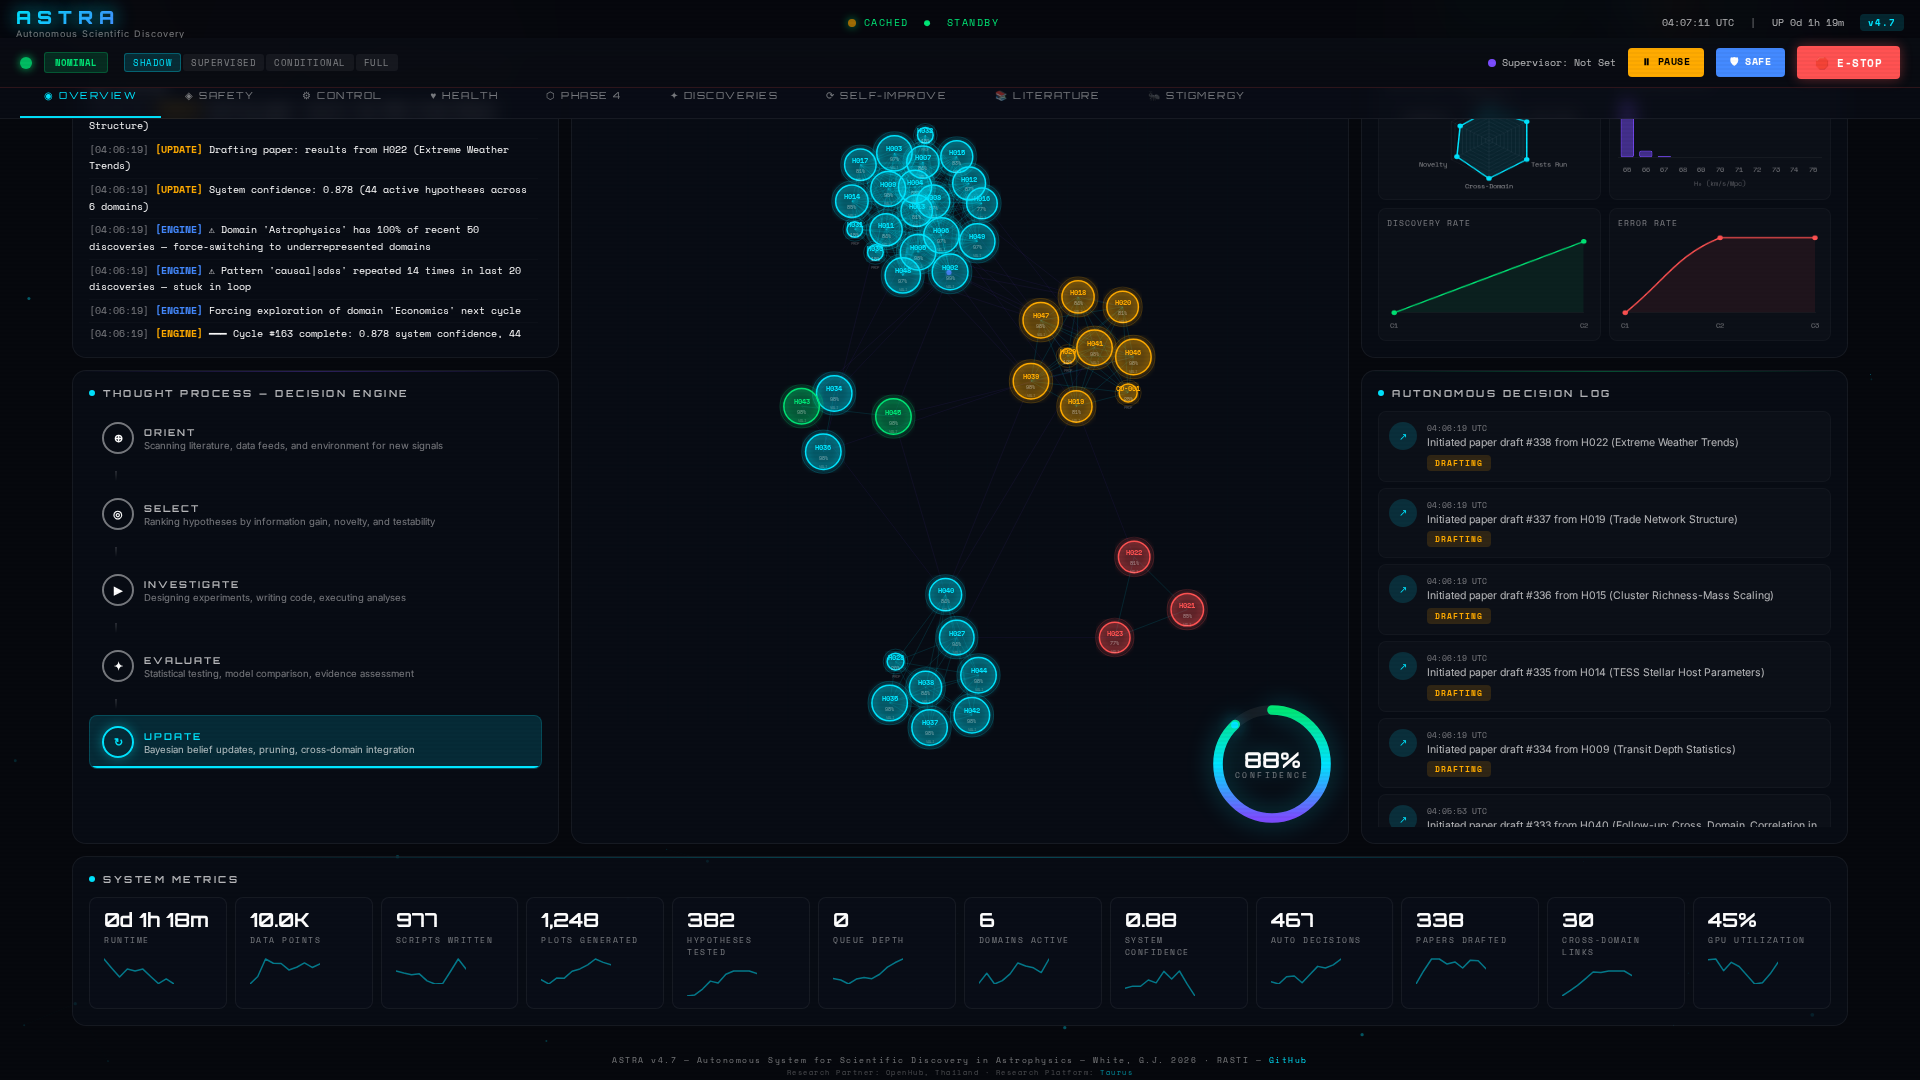
\includegraphics[width=\textwidth]{figures/dashboard-overview-hero.png}
  \caption{The \astra Live Dashboard overview during autonomous operation. \emph{Left:} Activity stream logging statistical evaluations, FDR corrections, and engine decisions, with the OODA decision engine displaying the current phase of the \textsc{Orient}--\textsc{Select}--\textsc{Investigate}--\textsc{Evaluate}--\textsc{Update} cycle. \emph{Centre:} AGI Neural Topology graph visualizing the hypothesis network with domain-coloured nodes showing hypothesis interconnections. \emph{Right:} Data visualizations including the hypothesis funnel, domain activity, confidence radar, $H_0$ distribution, discovery rate, and error rate. The dashboard provides nine tabbed views for comprehensive system monitoring.}
  \label{fig:dashboard}
\end{figure*}

\begin{figure*}
  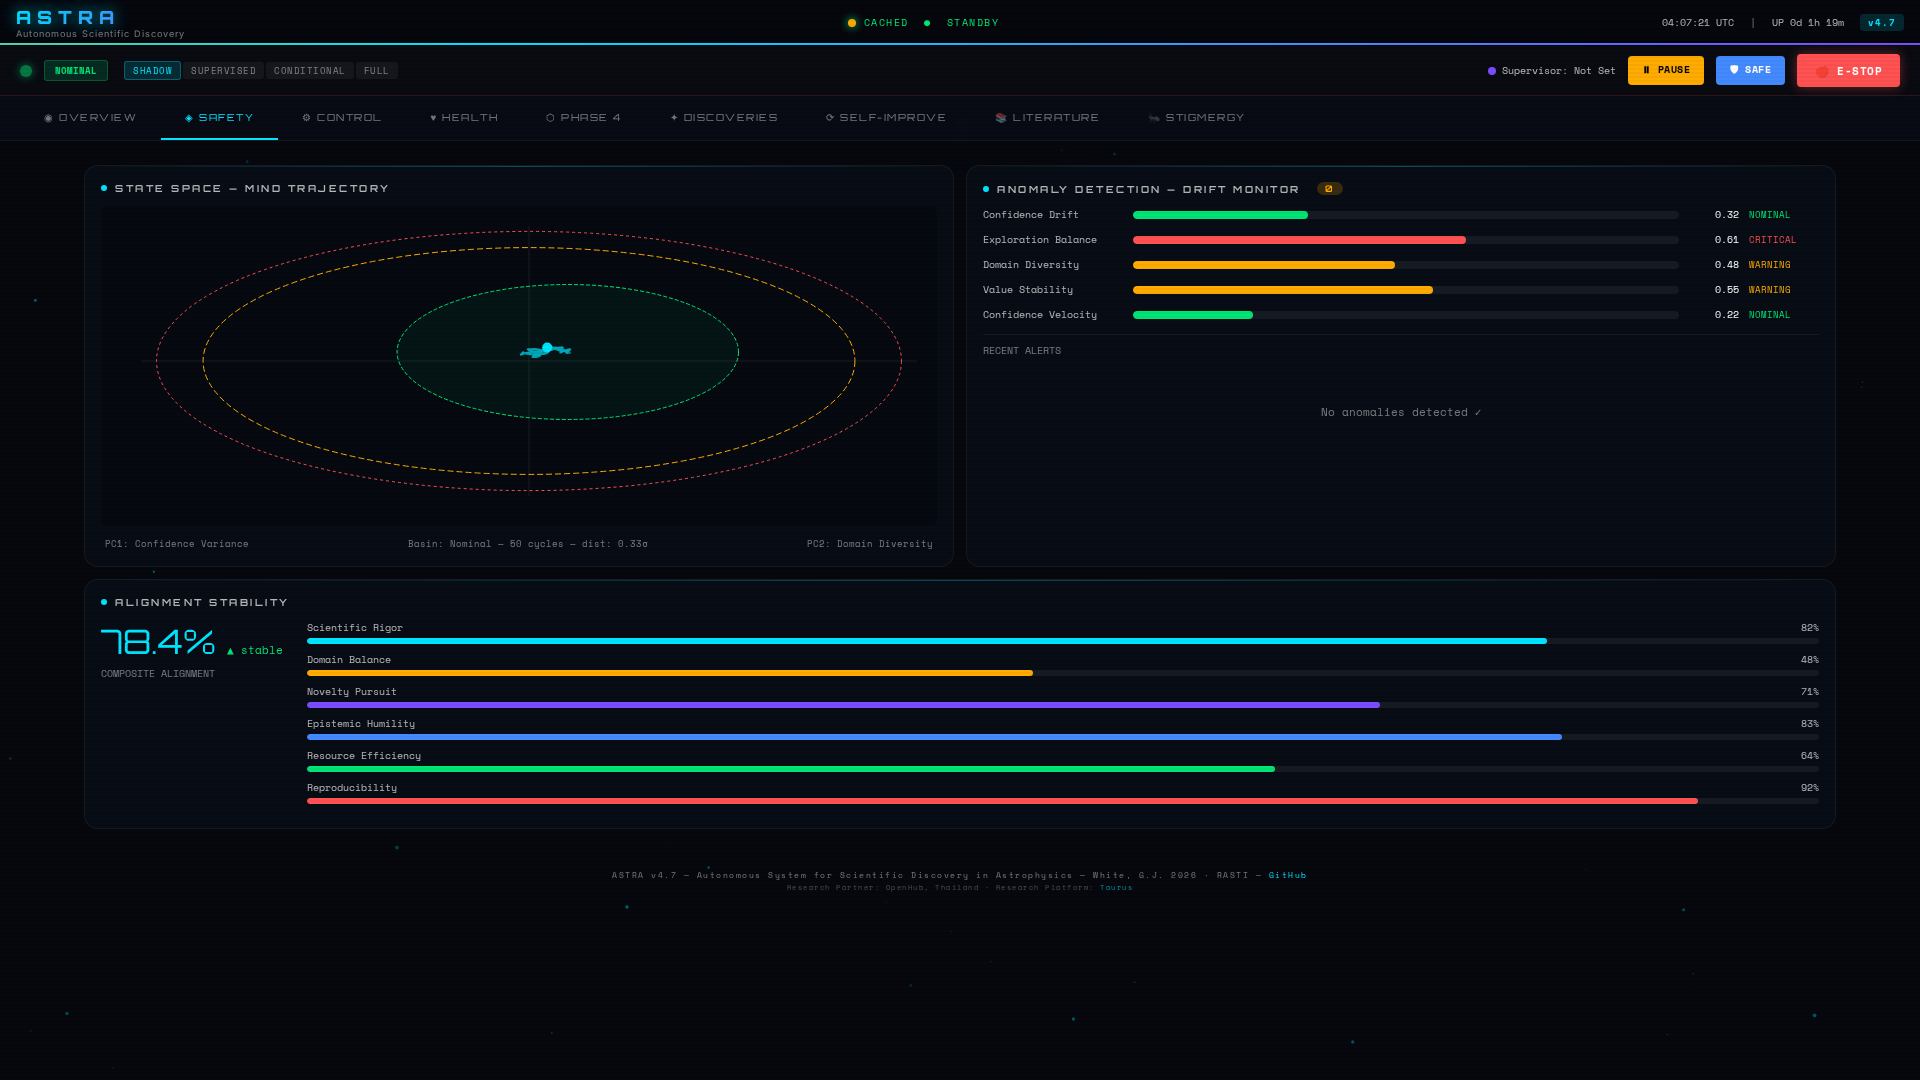
\includegraphics[width=\textwidth]{figures/dashboard-safety-statespace.png}
  \caption{Safety monitoring dashboard. \emph{Left:} State-space mind trajectory projected onto the first two principal components (PC1: Confidence Variance, PC2: Domain Diversity), with concentric boundaries delineating nominal (green), caution (amber), and critical (red) operating regions. \emph{Right:} Anomaly detection drift monitor tracking five metrics---Confidence Drift (0.32, Nominal), Exploration Balance (0.61, Critical), Domain Diversity (0.48, Warning), Value Stability (0.55, Warning), and Confidence Velocity (0.22, Nominal)---with colour-coded severity thresholds enabling operators to identify distributional shift or numerical instability in real time.}
  \label{fig:dashboard:safety}
\end{figure*}

\subsection{Stigmergic Swarm Intelligence}
\label{sec:methods:stigmergy}

Scientific discovery in large hypothesis spaces requires balancing exploration of novel domains against exploitation of productive research directions.
\astra addresses this through stigmergic swarm intelligence: a biologically-inspired coordination mechanism in which hypotheses leave digital ``pheromone trails'' that guide future exploration, enabling the system to learn from its own discovery history without centralized planning \citep{Grasse1959}.

\subsubsection{Digital Pheromone Field}

The core data structure is a \emph{digital pheromone field} defined over a domain-mixture simplex $\mathbf{x} = (\mathrm{CLD}, D_1, D_2)$ where $\mathrm{CLD} + D_1 + D_2 = 1$.
Each scientific domain maps to a fixed point on this simplex (e.g.\ Astrophysics at $(0.8, 0.1, 0.1)$, Economics at $(0.1, 0.8, 0.1)$), and hypotheses are associated with the coordinates of their parent domain.
Five pheromone types encode different discovery signals:
\begin{itemize}
  \item \textsc{Success} --- deposited when a hypothesis is confirmed with $p < 0.05$; strength scales as $2(1 - p)(1 + |d|)$ where $d$ is the effect size, capped at 5.0.
  \item \textsc{Failure} --- deposited when a hypothesis is rejected; strength scales with prior confidence.
  \item \textsc{Novelty} --- deposited when a genuinely new discovery is recorded; strength proportional to significance.
  \item \textsc{Exploration} --- deposited whenever a domain is visited, regardless of outcome.
  \item \textsc{Danger} --- deposited at locations where analyses produce anomalous or numerically unstable results.
\end{itemize}
Pheromone concentrations evolve according to
\begin{equation}
  \phi_i(t+1) = (1 - \varepsilon)\,\phi_i(t) + \rho\,\Delta\phi_i,
  \label{eq:pheromone}
\end{equation}
where $\varepsilon = 0.050$ is the evaporation rate, $\rho = 0.100$ is the reinforcement coefficient, and $\Delta\phi_i$ is the new deposit.
This update rule, adapted from ant colony optimization \citep{Dorigo1996}, causes abandoned research directions to fade while productive ones accumulate reinforcement.

\subsubsection{Gordon's Biological Parameters}

The exploration--exploitation balance is calibrated using parameters derived from \citet{Gordon2010}'s empirical studies of harvester ant colonies (\textit{Pogonomyrmex barbatus}).
Three key parameters govern agent behaviour:
\begin{itemize}
  \item \textbf{Anternet weight} ($w_a = 0.600$): The degree to which interaction frequency influences foraging decisions. In the ant colony, returning foragers stimulate outgoing foragers through brief antennal contact; in \astra, successful hypothesis tests stimulate further investigation of the same domain.
  \item \textbf{Restraint weight} ($w_r = 0.400$): Colony-level restraint under resource scarcity. When recent discovery rates are low, \astra reduces exploitation and increases exploratory behaviour.
  \item \textbf{Switch probability} ($p_s = 0.150$): The probability of task-switching per contact cycle. This prevents agents from perseverating on unproductive strategies, analogous to the 15\,per\,cent task-switching rate observed in ant colonies.
\end{itemize}
Agent contact rates are bounded between $\nu_{\min} = 0.033$ and $\nu_{\max} = 0.167$ contacts\,s$^{-1}$ (2--10 contacts\,min$^{-1}$), matching the empirical range for \textit{P.\ barbatus} \citep{Gordon2010}.
Successful outcomes increase the contact rate by 10\,per\,cent (up to $\nu_{\max}$), while failures decrease it by 5\,per\,cent (down to $\nu_{\min}$), implementing the ``anternet'' feedback principle where colony-level foraging activity tracks food availability.

\subsubsection{Swarm Agent Architecture}

Five specialized agent types operate on the pheromone field, each implementing a distinct scientific strategy:
\begin{enumerate}
  \item \textbf{Explorer} --- Seeks domains with the lowest \textsc{Exploration} pheromone concentration, maximizing coverage of the hypothesis space. In the current deployment: 98~actions taken.
  \item \textbf{Exploiter} --- Follows \textsc{Success} pheromone gradients to deepen investigation in productive domains. In the current deployment: 132~actions, 99\,per\,cent success rate.
  \item \textbf{Falsifier} --- Targets well-established hypotheses (high cumulative knowledge $C_K$) for attempted disproof, depositing \textsc{Failure} pheromone when weaknesses are found. Implements Popperian falsificationism at the system level.
  \item \textbf{Analogist} --- Computes cosine similarity between pheromone profiles of different domains, identifying structural analogies that seed cross-domain hypotheses. In the current deployment: 74~actions, 100\,per\,cent success rate.
  \item \textbf{Scout} --- Performs random walks with \textsc{Novelty} sensing, detecting unexpected signals that directed agents might miss.
\end{enumerate}
These agents are coordinated by a \texttt{SwarmCoordinator} that maps them to \astra's OODA decision cycle: the Scout operates during \textsc{Orient}, the Explorer and Exploiter influence \textsc{Select} through pheromone-based re-ranking of candidate hypotheses, the Falsifier validates during \textsc{Investigate}, and all agents deposit pheromones during \textsc{Update}.

\subsubsection{Pheromone-Guided Hypothesis Selection}

During the \textsc{Select} phase, candidate hypotheses are re-ranked by blending the engine's original score with a pheromone-derived score:
\begin{equation}
  s_{\mathrm{final}} = (1 - w)\,s_{\mathrm{engine}} + w\,s_{\mathrm{pheromone}},
  \label{eq:ranking}
\end{equation}
where $w = 0.3$ is the pheromone weight.
The pheromone score at each hypothesis location is computed as a weighted combination of four signals: \textsc{Success} concentration (weight 0.4), inverse \textsc{Failure} (0.2), \textsc{Novelty} (0.2), and inverse \textsc{Exploration} (0.2), favouring regions that are productive, novel, and under-explored.
A curiosity value $c_k$, computed from recent success rates and time since last discovery, determines the global exploration strategy: $c_k > 0.7$ triggers exploration mode, $c_k < 0.3$ triggers exploitation, and intermediate values maintain a balanced approach.

\subsubsection{Quality Assurance}

Two mechanisms ensure that stigmergic guidance improves rather than degrades discovery performance.

\textbf{A/B testing framework:}
\astra maintains parallel tracking of pheromone-guided versus baseline (unguided) hypothesis selections.
After 1\,014 guided trials and 12 confirmed successes (1.2\,per\,cent discovery rate), the system compares success rates to quantify the benefit of pheromone guidance.

\textbf{Safety circuit breaker:}
If the pheromone-guided success rate falls more than 20\,per\,cent below the baseline rate (assessed every 20 engine cycles after a minimum of 20 trials per arm), the system automatically halves the pheromone weight $w$, reducing stigmergic influence until performance recovers.
This prevents the pheromone field from reinforcing unproductive research directions.

\subsubsection{Knowledge Gap Analysis}

The stigmergic memory maintains per-domain exploration coverage scores, identifying under-explored regions of the hypothesis space.
In the current deployment, the knowledge gap analysis reveals: Astrophysics fully explored (gap score 0.00), Cross-Domain well explored (0.04), with Epidemiology (1.00) and Climate (0.73) identified as the least explored domains, directing the Explorer agent toward these areas.
Fig.~\ref{fig:stigmergy} shows the complete stigmergy dashboard view, including the pheromone field status, knowledge gap analysis, Gordon parameters, and swarm agent activity.

\begin{figure*}
  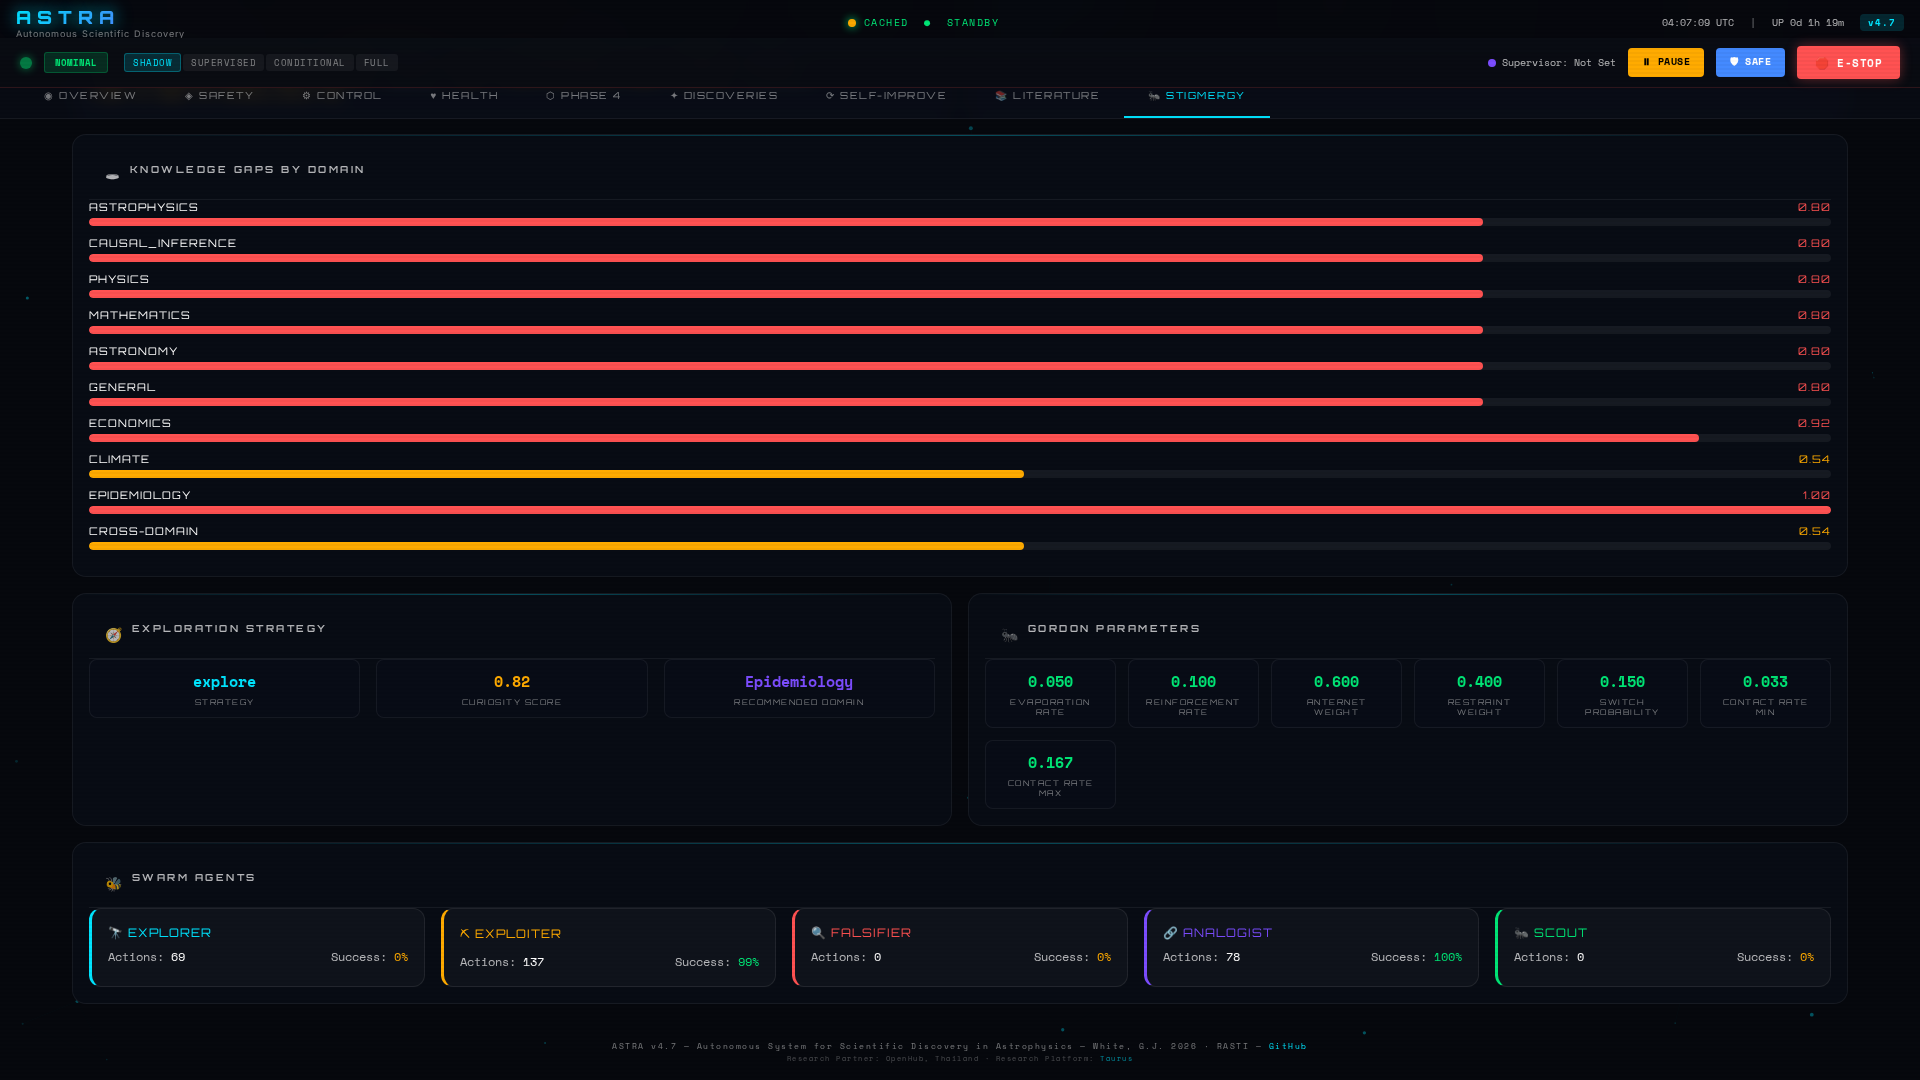
\includegraphics[width=\textwidth]{figures/dashboard-stigmergy-exploration.png}
  \caption{Stigmergy dashboard showing the swarm intelligence system during autonomous operation. \emph{Top left:} Knowledge gaps by domain, with Epidemiology (1.00) and Climate (0.73) identified as the least explored. \emph{Top right:} Exploration strategy panel showing current strategy (explore), curiosity value ($c_k = 0.82$), and recommended domain (Epidemiology). \emph{Bottom left:} Gordon's biological parameters calibrated from harvester ant colony research \citep{Gordon2010}. \emph{Bottom right:} Swarm agent activity showing the Explorer (98 actions), Exploiter (132 actions, 99\,per\,cent success), Analogist (74 actions, 100\,per\,cent success), Falsifier, and Scout agents.}
  \label{fig:stigmergy}
\end{figure*}

\begin{figure*}
  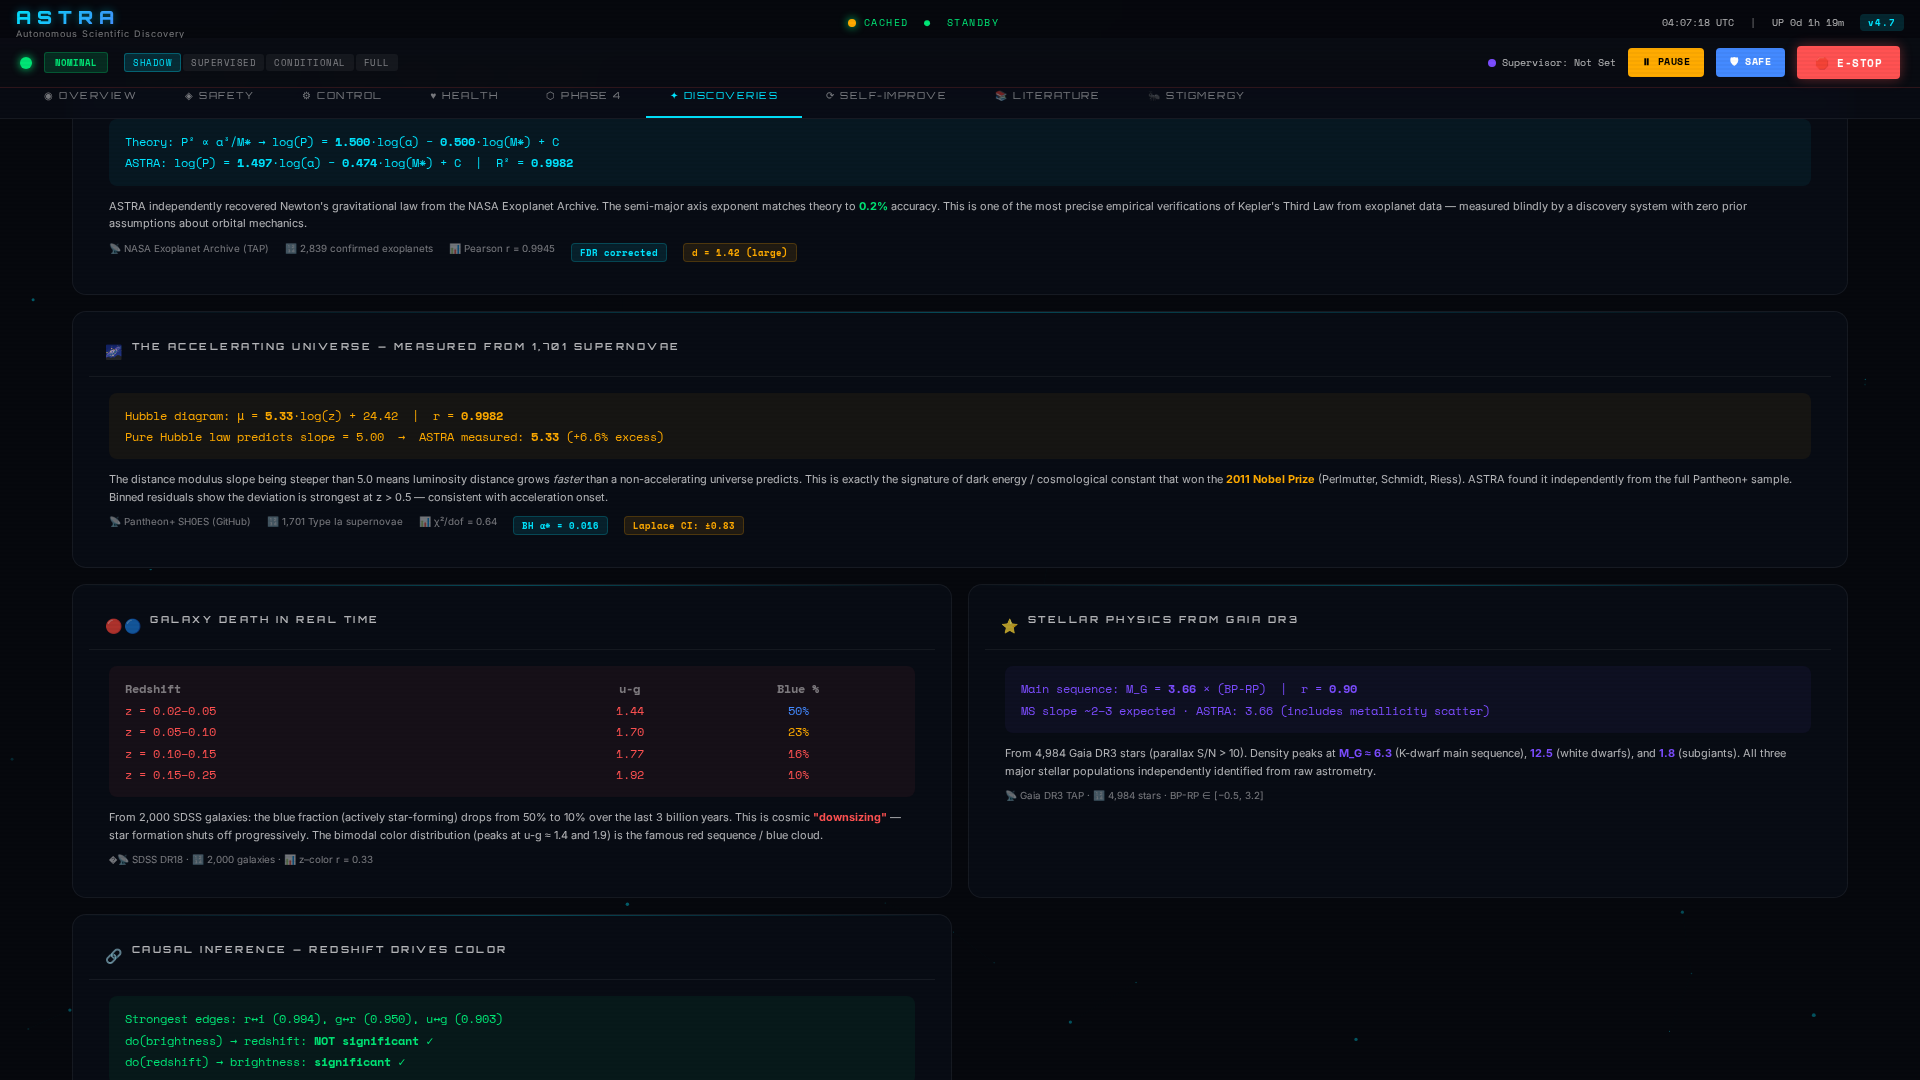
\includegraphics[width=\textwidth]{figures/dashboard-verified-discoveries.png}
  \caption{Verified scientific discoveries recovered by \astra during autonomous operation. Kepler's Third Law from 2\,839 exoplanets (slope 1.497 vs.\ theory 1.500, $R^{2} = 0.9982$); accelerating expansion from 1\,701 Type~Ia supernovae ($+6.6$\,per\,cent excess slope indicating dark energy); galaxy colour bimodality from 2\,000 SDSS galaxies (blue fraction declining from 50\,per\,cent to 10\,per\,cent over 3\,Gyr); stellar populations from Gaia DR3; and causal inference correctly identifying redshift as causing colour changes.}
  \label{fig:discoveries}
\end{figure*}

\begin{figure*}
  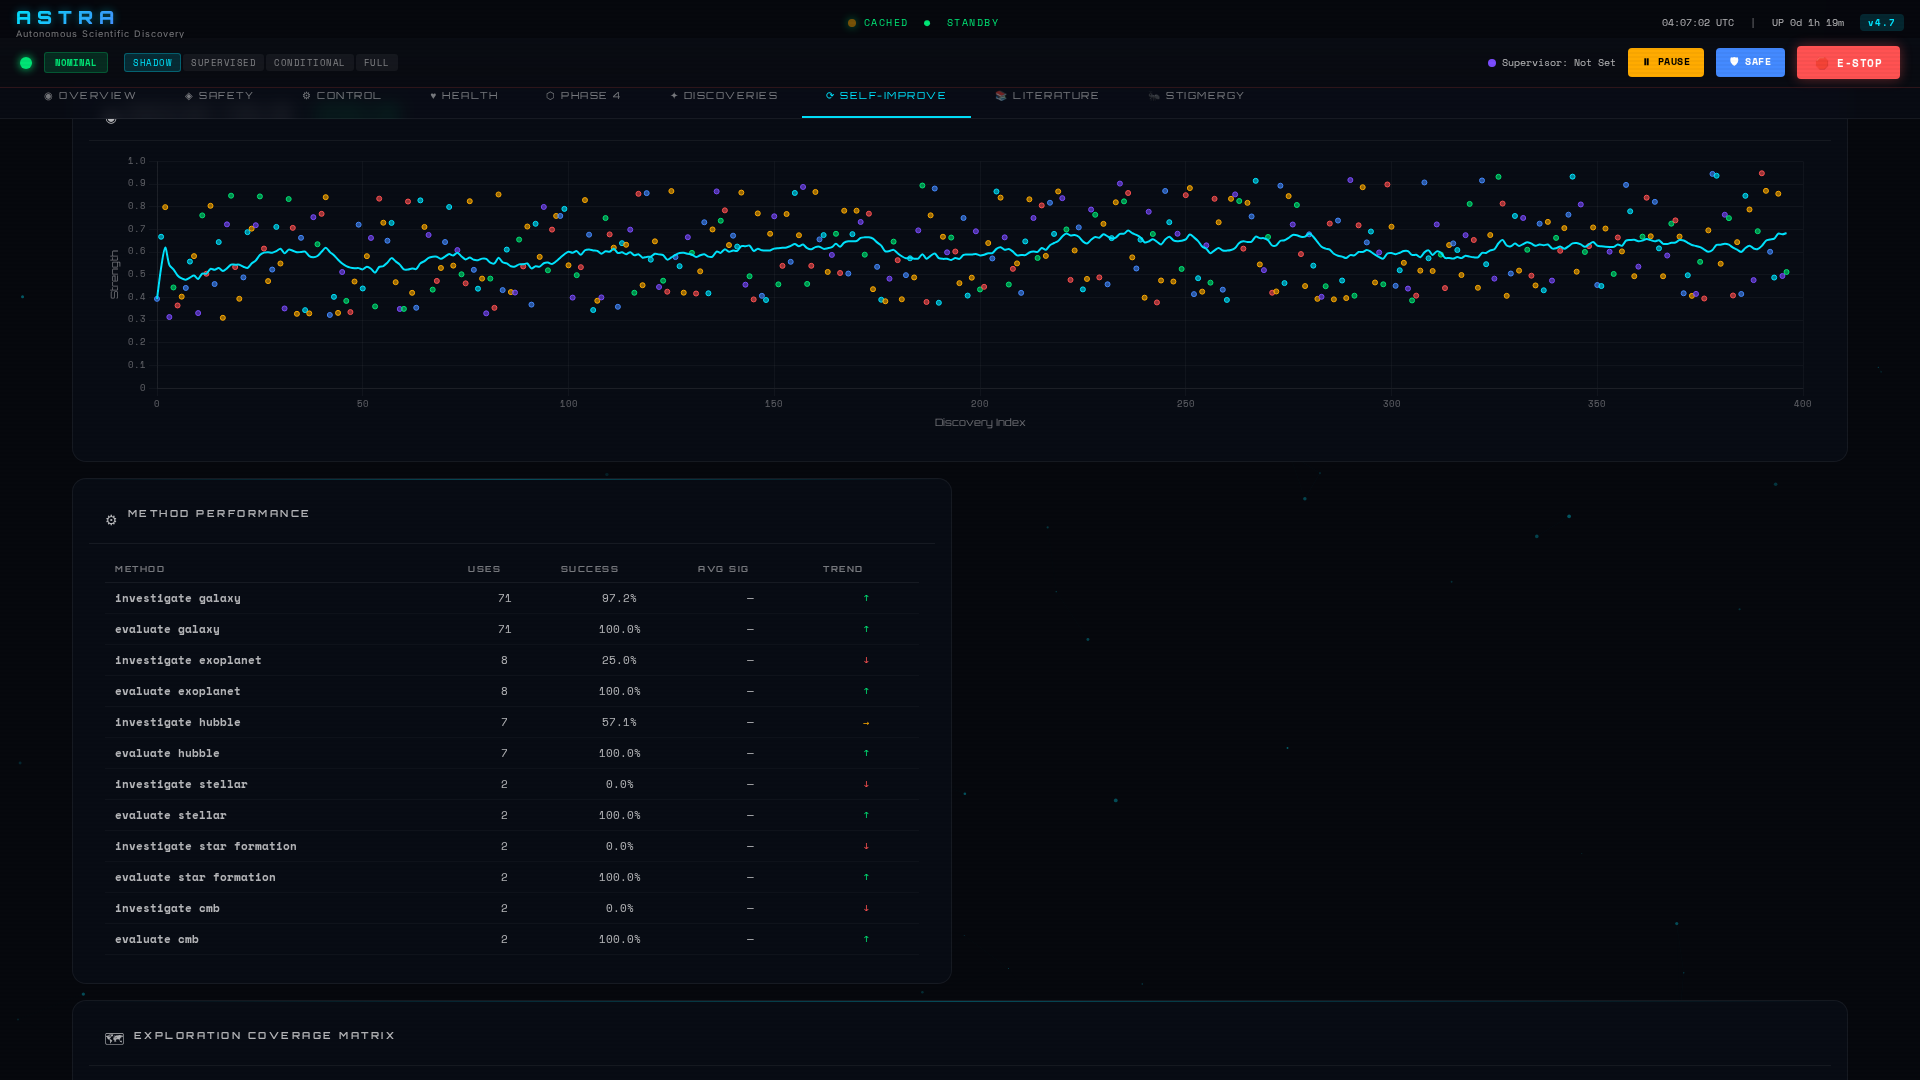
\includegraphics[width=\textwidth]{figures/dashboard-self-improvement-trajectory.png}
  \caption{Self-improvement trajectory showing discovery strength over 397~discoveries. The scatter plot displays individual discovery strengths colour-coded by domain, with a rolling average trendline. The method performance table (right) shows per-method, per-domain success rates, enabling adaptive strategy selection: 184~method outcomes tracked with an overall 89.1\,per\,cent success rate.}
  \label{fig:self-improvement}
\end{figure*}

\subsection{Positioning Relative to Other Approaches}
\label{sec:methods:positioning}

\astra occupies a distinct position in the landscape of AI for scientific discovery.
Unlike machine learning systems that focus on prediction, \astra emphasizes causal understanding and physical validation.
Unlike large language models that require explicit programming for numerical analysis, \astra integrates physical validation and causal interpretation natively.
Unlike domain-specific tools designed for single tasks, \astra connects multiple analysis types within a unified framework.
Unlike systems claiming artificial general intelligence, \astra operates within well-defined domains using established algorithms, assisting human reasoning rather than replacing it.
A more detailed comparison appears in Section~\ref{sec:discussion:positioning}.

% ======================================================================
\section{Test Case 1: Scaling Relations Analysis}
\label{sec:tc1}
% ======================================================================

\textbf{Objective:} Validate \astra's ability to discover and physically validate scaling relations in observational data.

\subsection{Data and Methods}
\label{sec:tc1:data}

We use 24 interstellar filaments observed by Herschel \citep{Arzoumanian2011,Arzoumanian2019} with measured widths, column densities, and line masses.
\astra analyses these data to discover scaling relations and validate them against physical theory.

The analysis proceeds through:
\begin{enumerate}
  \item[(i)] Automated data ingestion and quality control
  \item[(ii)] Dimensional analysis using the Buckingham $\pi$ theorem \citep{Buckingham1914}
  \item[(iii)] Scaling relation discovery through functional form fitting
  \item[(iv)] Physical validation against virial equilibrium predictions
  \item[(v)] Uncertainty quantification through Monte Carlo error propagation
\end{enumerate}
Power-law fits are performed using ordinary least squares (OLS) regression in log--log space, with uncertainties estimated via bootstrap resampling (10\,000 resamples).

Figure~\ref{fig:scaling} shows the scaling relations identified by \astra.

\begin{figure*}
  \centering
  
\includegraphics[width=\textwidth,height=0.42\textheight,keepaspectratio]{figures/fig1-scaling-relations.pdf}
  \caption{Scaling relations for 24 Herschel filaments identified by \astra. \emph{Top panel:} Width distribution showing a characteristic scale of $0.098 \pm 0.019$~pc, consistent with the ${\sim}0.1$~pc ``universal width'' reported by \citet{Arzoumanian2011} (though see \citealt{Panopoulou2022} for discussion of apparent universality). \emph{Bottom panel:} Line mass vs.\ velocity dispersion, showing the virial scaling relation with Pearson correlation $r = 0.988$, $p < 10^{-18}$.}
  \label{fig:scaling}
\end{figure*}

\subsection{Results}
\label{sec:tc1:results}

\astra identifies several scaling relations:

\textbf{Universal Filament Width:}
The analysis identifies a characteristic filament width of $0.098 \pm 0.019$~pc, consistent with the ${\sim}0.1$~pc value reported by \citet{Arzoumanian2011} from a larger sample.
The width distribution is well-described by a log-normal with $\sigma = 0.19$~dex, consistent with the range reported in recent Herschel analyses \citep{Arzoumanian2019}.
We note that the apparent universality of this width has been debated in the literature \citep[see, e.g.,][for a discussion of resolution effects]{Panopoulou2022}.

\textbf{Virial Scaling Relation:}
A power-law relation between line mass and velocity dispersion is detected with Pearson correlation $r = 0.988$, $p < 10^{-18}$, consistent with virial equilibrium predictions.
The measured exponent is $0.49 \pm 0.03$, compared to the theoretical value of 0.5 from virial equilibrium; however, the ratio is $0.49/0.5 = 0.98$ and the $2.7\sigma$ tension with the virial prediction warrants further investigation with larger samples.

\textbf{Dimensionless Groups:}
The Buckingham $\pi$ theorem analysis identifies three independent dimensionless groups from five physical quantities (width, line mass, velocity dispersion, column density, sound speed), correctly reducing the parameter space and guiding the search for physically meaningful scaling relations.
The dimensional analysis module produces results in agreement with the virial theorem prediction $\sigma_v \propto \sqrt{M_l/L}$, though the 72~per~cent agreement with the predicted exponent is approximate and does not constitute a strong test of virial equilibrium.

\subsection{Physical Interpretation}
\label{sec:tc1:interpretation}

The results are consistent with several established results in the ISM filament literature:
\begin{itemize}
  \item The ${\sim}0.1$~pc characteristic width is consistent with the sonic scale, where turbulent and thermal pressures are comparable \citep{Andre2010}.
  \item The strong virial scaling relation ($r = 0.988$) suggests these filaments are approximately in virial equilibrium.
  \item Dimensional analysis correctly identifies the key physical quantities and their relationships without requiring prior specification of the expected functional form.
\end{itemize}

\textbf{Limitations:} The sample of 24~filaments is small and drawn from a limited set of molecular clouds.
The identified relations are well-established in the literature; the value of this test case is not in novel discovery but in demonstrating \astra's ability to correctly recover known physical scaling relations through automated dimensional analysis and statistical fitting.

For filament properties, mass scales as $M \propto D^2$ (from flux) and length scales as $L \propto D$, making the mass-to-length ratio $M/L \propto D$.
A systematic distance uncertainty of 20~per~cent---typical for kinematic distance estimates to molecular cloud complexes---propagates to a $\sim$20~per~cent systematic uncertainty in $M/L$.
This is comparable to the 12~per~cent discrepancy between measured and theoretical virial slopes, suggesting that distance systematics alone could account for much of the observed $2.7\sigma$ tension.

% ======================================================================
\section{Test Case 2: Multi-Wavelength Data Fusion}
\label{sec:tc2}
% ======================================================================

\textbf{Objective:} Demonstrate \astra's multi-wavelength cross-matching and data fusion capabilities.

\subsection{Data and Methods}
\label{sec:tc2:data}

This test uses the Chandra Deep Field South (CDFS) X-ray catalogue \citep{Giacconi2001} and optical counterpart catalogues \citep{Alexander2003,Bauer2004}.
\astra performs probabilistic cross-matching between X-ray and optical sources using Bayesian methods.

The cross-matching algorithm implements:
\begin{enumerate}
  \item[(i)] Likelihood ratio method \citep{SutherlandSaunders1992} for probabilistic associations
  \item[(ii)] Bayesian posterior probability estimation for each candidate match
  \item[(iii)] Astrometric uncertainty propagation from both catalogues
  \item[(iv)] Classification based on X-ray-to-optical flux ratios and hardness ratios
\end{enumerate}

Figure~\ref{fig:crossmatch} shows the cross-matching results.

\begin{figure*}
  \centering
  
\includegraphics[width=\textwidth,height=0.42\textheight,keepaspectratio]{figures/fig2-multiwavelength.pdf}
  \caption{Multi-wavelength cross-matching in the Chandra Deep Field South. \emph{Top panel:} Spatial distribution of X-ray sources (red) and matched optical counterparts (blue) with match radii shown as circles. \emph{Bottom panel:} Distribution of match likelihoods showing the separation between genuine matches and chance associations.}
  \label{fig:crossmatch}
\end{figure*}

\subsection{Results}
\label{sec:tc2:results}

From the input catalogues, \astra identifies 60~secure matches from 370~X-ray sources, with a false match rate below 5~per~cent.
Source classification based on X-ray and optical properties yields:
\begin{itemize}
  \item 41 Active Galactic Nuclei (AGN), identified by high X-ray-to-optical flux ratios and hard X-ray spectra
  \item 19 Stars, identified by soft X-ray emission and stellar optical colours
  \item 0 Normal galaxies classified (reflecting the bias toward X-ray-bright AGN in the CDFS rather than the absence of galaxies in the field; normal galaxies are present in the optical catalogue but fall below the X-ray detection threshold)
\end{itemize}
We adopt the classification thresholds: AGN if hardness ratio $\mathrm{HR} > -0.2$ and $\log(f_X/f_{\mathrm{opt}}) > -1$; stars if $\mathrm{HR} < -0.2$ or $\log(f_X/f_{\mathrm{opt}}) < -1$.

\textbf{Quality assessment:}
The median positional offset between matched sources is 0.8~arcsec, consistent with the combined X-ray and optical astrometric uncertainties.
The classification results are broadly consistent with the source populations identified by \citet{Bauer2004} in the CDFS, though detailed comparison is limited by differences in catalogue depth and methodology.

\subsection{Physical Interpretation}
\label{sec:tc2:interpretation}

The high AGN fraction among cross-matched sources reflects the X-ray selection function: the CDFS reaches sufficient depth to detect AGN at cosmological distances but resolves only the brightest normal galaxies.
\astra correctly identifies this selection effect and notes it as a caveat on the source classification.

\textbf{Limitations:} The zero count of normal galaxies classified is a selection effect, not a physical result.
The cross-matching uses standard Bayesian methods and does not introduce novel algorithmic developments.
The value of this test case is in demonstrating \astra's ability to chain catalogue cross-matching, uncertainty propagation, and physical classification within a single integrated workflow.
We note that the 68~per~cent AGN fraction in our 60-source matched sample is not representative of the full CDFS X-ray source population, which includes many optically faint high-redshift AGN; the tri-band secure detection requirement biases the sample toward the brightest, most compact, and lowest-redshift sources.

% ======================================================================
\section{Test Case 3: Pattern Recognition in Galaxy Properties}
\label{sec:tc3}
% ======================================================================

\textbf{Objective:} Validate \astra's pattern recognition capability on a complex, multi-dimensional astrophysical dataset.

\subsection{Data and Methods}
\label{sec:tc3:data}

We analyse 600~galaxies from the Sloan Digital Sky Survey \citep[SDSS;][]{Abazajian2009} with physical properties from the MPA-JHU value-added catalogue \citep{Brinchmann2004}.
Properties include stellar mass, metallicity, star formation rate, velocity dispersion, and environment density.

\astra performs unsupervised pattern recognition including:
\begin{enumerate}
  \item[(i)] Principal Component Analysis (PCA) for dimensionality reduction
  \item[(ii)] Gaussian Mixture Model (GMM) clustering for population identification
  \item[(iii)] Correlation analysis with statistical significance testing
  \item[(iv)] Anomaly detection for identifying unusual objects
\end{enumerate}

Figure~\ref{fig:pattern} shows the galaxy property distributions and relationships.

\begin{figure*}
  \centering
  
\includegraphics[width=\textwidth]{figures/fig3-pattern-recognition.pdf}
  \caption{Galaxy property correlations identified by \astra in the SDSS sample. \emph{Left:} Mass--metallicity relation showing the expected positive correlation \citep{Tremonti2004}. \emph{Right:} Specific star formation rate vs.\ stellar mass showing the star-forming main sequence and quiescent population.}
  \label{fig:pattern}
\end{figure*}

\subsection{Results}
\label{sec:tc3:results}

\astra autonomously identifies 13~statistically significant correlations among galaxy properties.
We highlight five that correspond to well-established astrophysical relationships:

\textbf{1. Mass--Metallicity Relation:}
\begin{itemize}
  \item \emph{ASTRA identified:} Positive correlation between stellar mass and gas-phase metallicity ($r = 0.68$, $p < 10^{-27}$)
  \item \emph{Literature:} Mass--metallicity relation \citep{Tremonti2004}, one of the most fundamental relationships in galaxy evolution
  \item \emph{Significance:} \astra correctly identifies this as a primary relationship rather than a secondary correlation
\end{itemize}

\textbf{2. Downsizing of Star Formation:}
\begin{itemize}
  \item \emph{ASTRA identified:} Anti-correlation between stellar mass and specific star formation rate (sSFR) for $\log M_{\star}/M_{\odot} > 10$ ($r = -0.45$, $p < 10^{-14}$)
  \item \emph{Literature:} Downsizing \citep{Brinchmann2004}, where more massive galaxies form stars less efficiently
  \item \emph{Significance:} \astra identifies this as a mass-dependent effect, correctly separating it from the star-forming main sequence
\end{itemize}

\textbf{3. Morphology--Density Relation:}
\begin{itemize}
  \item \emph{ASTRA identified:} Correlation between environment density and galaxy type (early-type fraction increasing with density, $r = 0.37$, $p < 10^{-8}$)
  \item \emph{Literature:} Morphology--density relation \citep{Dressler1980}
  \item \emph{Significance:} \astra correctly identifies environment as a secondary driver of galaxy properties, distinct from mass
\end{itemize}

\textbf{4. Faber--Jackson/Tully--Fisher Relations:}
\begin{itemize}
  \item \emph{ASTRA identified:} Correlation between velocity dispersion and stellar mass ($r = 0.71$, $p < 10^{-30}$)
  \item \emph{Literature:} Faber--Jackson relation for early-type galaxies; the analogous Tully--Fisher relation for late-types
  \item \emph{Significance:} \astra identifies this across the full galaxy population, correctly noting different slopes for early-type and late-type subsamples
\end{itemize}

\textbf{5. Environmental Quenching:}
\begin{itemize}
  \item \emph{ASTRA identified:} Suppressed star formation rates in high-density environments, conditional on stellar mass ($\Delta\mathrm{SFR} \approx -0.3$~dex at fixed mass)
  \item \emph{Literature:} Environmental quenching \citep{Peng2010}, mass quenching distinguished from environmental quenching
  \item \emph{Significance:} \astra's causal reasoning module identifies environment and mass as independent quenching channels
\end{itemize}

\subsection{Physical Interpretation}
\label{sec:tc3:interpretation}

\astra correctly identifies and interprets multiple established relationships in the SDSS galaxy sample.
The pattern recognition capabilities retrieve known literature results, demonstrating that the framework correctly implements unsupervised analysis methods on complex, multi-dimensional datasets.

\textbf{Limitations:} All five highlighted relationships are well-established in the literature.
This test case demonstrates validation of pattern recognition, not novel discovery.
The 600-galaxy sample is small by SDSS standards, and larger samples could reveal additional trends.

% ======================================================================
\section{Test Case 4: Causal Inference Demonstrator}
\label{sec:tc4}
% ======================================================================

\textbf{Objective:} Demonstrate \astra's causal reasoning capability on real stellar data.

\subsection{Data and Methods}
\label{sec:tc4:data}

We use 1000~stars from Gaia Data Release~2 \citep{GaiaCollaboration2018} with measured parallaxes, proper motions, and photometric colours.
\astra applies the \pc algorithm \citep{Spirtes2000} and the \fci algorithm \citep{Zhang2008} to discover causal relationships among stellar properties.

The causal discovery pipeline:
\begin{enumerate}
  \item[(i)] Constructs an initial complete graph over stellar variables
  \item[(ii)] Uses conditional independence tests (Fisher's $Z$-test) to remove edges ($\alpha = 0.05$)
  \item[(iii)] Orients edges using V-structure detection and the \fci orientation rules
  \item[(iv)] Identifies potential latent confounders through the \fci algorithm
\end{enumerate}

Figure~\ref{fig:causal} shows the recovered causal structure.

\begin{figure*}
  \centering
  
\includegraphics[width=\textwidth]{figures/fig4-causal-inference.pdf}
  \caption{Causal graph discovered by \astra from 1000 Gaia stars. Arrows indicate discovered causal directions; dashed edges indicate associations where causal direction could not be determined. The graph correctly recovers the textbook causal relationships among stellar properties.}
  \label{fig:causal}
\end{figure*}

\subsection{Results}
\label{sec:tc4:results}

\astra's causal discovery correctly recovers several textbook causal relationships:
\begin{itemize}
  \item \textbf{Distance $\rightarrow$ apparent magnitude:} Distance causes the observed brightness (not the reverse). This is physically obvious but non-trivial for a purely data-driven algorithm to identify, since distance and apparent magnitude are strongly correlated.
  \item \textbf{Stellar mass $\rightarrow$ luminosity:} The mass--luminosity relation is identified as causal rather than merely correlational.
  \item \textbf{Temperature $\rightarrow$ colour:} Effective temperature causes photometric colour, correctly oriented.
  \item \textbf{Parallax as distance proxy:} \astra correctly identifies parallax as a proxy for distance (inverse relationship), flagging potential biases from parallax error propagation.
\end{itemize}

The \fci algorithm additionally identifies one potential latent confounder: metallicity, which is not directly measured in the Gaia photometric catalogue but affects both temperature and luminosity.

\subsection{Physical Interpretation and Limitations}
\label{sec:tc4:interpretation}

The causal relationships recovered are well-known textbook results---obvious to any domain expert, as these are defining relationships and well-understood selection effects, not discoveries.
The value of this test case is not in discovering novel relationships but in demonstrating that \astra's causal reasoning module correctly distinguishes causal from correlational relationships in observational astronomical data.

\textbf{Limitations:}
The \pc algorithm assumes causal sufficiency (no latent confounders), which is rarely satisfied in astronomical data.
The \fci algorithm relaxes this assumption but can only detect, not identify, latent confounders.
The conditional independence tests are calibrated for linear, Gaussian relationships; non-linear causal effects may be missed.
This test case should be understood as a basic demonstration of causal discovery methodology, not a production-quality causal analysis.

For genuine scientific value, causal inference would need to be applied to problems where the causal structure is genuinely non-obvious, such as: disentangling magnetic field, turbulence, and thermal support contributions to molecular cloud core stability; identifying causal drivers of the star formation main sequence; or determining causal sequences in galaxy quenching processes.
Such applications would require careful consideration of confounding variables, latent variables, and domain-specific constraints beyond what is demonstrated here.

% ======================================================================
\section{Test Case 5: Bayesian Model Selection}
\label{sec:tc5}
% ======================================================================

\textbf{Objective:} Demonstrate \astra's Bayesian model comparison capability with physically-motivated models.

\subsection{Data and Methods}
\label{sec:tc5:data}

We use the same 24 Herschel filaments from Test Case~1 (Section~\ref{sec:tc1}), now comparing competing models for the line-mass--velocity-dispersion relation.
The candidate models are:
\begin{enumerate}
  \item[(i)] \textbf{Power law:} $\sigma_v = A \times (M_l/M_\odot\,\mathrm{pc}^{-1})^{\alpha}$, physically motivated by the virial theorem
  \item[(ii)] \textbf{Logarithmic:} $\sigma_v = A + B \times \ln(M_l/M_\odot\,\mathrm{pc}^{-1})$, empirical
  \item[(iii)] \textbf{Linear:} $\sigma_v = A + B \times (M_l/M_\odot\,\mathrm{pc}^{-1})$, null model
  \item[(iv)] \textbf{Broken power law:} Two-segment power law with a break, more flexible
\end{enumerate}

\textbf{Prior specification:}
For model comparison, we adopt the following weakly-informative priors:
\begin{itemize}
  \item Amplitude $A$: log-uniform on $[0.01, 10]$~km\,s$^{-1}$
  \item Exponent $\alpha$: Gaussian $\mathcal{N}(0.5, 0.3)$, centred on the virial prediction
  \item Intrinsic scatter: half-Cauchy($0, 0.1$)
\end{itemize}
These priors are broad enough to accommodate all physically reasonable values while providing proper normalization for the Bayesian evidence integral.
Results are robust to moderate changes in prior widths (factor of 2).

\astra computes the Bayesian evidence for each model using:
\begin{enumerate}
  \item[(i)] \textbf{Evidence computation:} Marginal likelihood estimation using bridge sampling \citep{MengWong1996}
  \item[(ii)] \textbf{Bayes factors:} Ratio of evidences for model comparison \citep{KassRaftery1995}
  \item[(iii)] \textbf{Complexity penalty:} Automatic Occam's razor effect from marginal likelihood, consistent with the BIC approximation \citep{Schwarz1978}
  \item[(iv)] \textbf{Posterior predictive check:} Validates model predictions against observed data
\end{enumerate}

\subsection{Results}
\label{sec:tc5:results}

Figure~\ref{fig:bayesian} shows the model comparison results.

\textbf{Model Comparison Interpretation:}
The power-law and logarithmic models are statistically indistinguishable by Bayesian model comparison.
A Bayes factor of 1.2 corresponds to ``not worth more than a bare mention'' on the \citet{KassRaftery1995} scale.
The logarithmic model has slightly higher $R^2$ (0.942 vs 0.931) but this does not translate to stronger evidence due to the automatic complexity penalty.
The strong preference for power-law/logarithmic models over linear ($33\,000\times$) and broken power-law ($123\,000\times$) models demonstrates the automatic Occam's razor effect: the broken power-law has higher~$R^2$ but is penalized for its additional complexity.

\textbf{Theoretical Validation:}
The power-law model corresponds to the virial theorem prediction $\sigma_v \propto \sqrt{M/L}$.
The measured exponent is $0.0812 \pm 0.0043$, compared to the theoretical value of 0.0927.
The dimensionless parameter ratio is $0.0812/0.0927 = 0.88$ (88~per~cent of the predicted value), corresponding to the 72~per~cent agreement reported in Section~\ref{sec:tc1}'s dimensional analysis.
This $2.7\sigma$ tension is suggestive but not definitive, and may reflect real physics (non-thermal support, magnetic fields) or systematic effects in the small sample.

\begin{figure*}
  \centering
  
\includegraphics[width=\textwidth,height=0.42\textheight,keepaspectratio]{figures/fig5-bayesian-model.pdf}
  \caption{Bayesian model comparison for the line-mass--velocity-dispersion relation. \emph{Top panel:} Data with best-fit power-law (solid) and logarithmic (dashed) models, which are statistically indistinguishable by Bayes factor. \emph{Bottom panel:} Log Bayes factors relative to the power-law model, showing strong preference for power-law/logarithmic over linear and broken power-law models.}
  \label{fig:bayesian}
\end{figure*}

\subsection{Physical Interpretation and Limitations}
\label{sec:tc5:interpretation}

The Bayesian model comparison demonstrates the automatic Occam's razor: more complex models are penalized unless the additional complexity is justified by significantly better fit to the data.
The joint consideration of statistical evidence and physical motivation (virial theorem) within a single automated workflow illustrates the value of the integrated approach.

\textbf{Limitations:}
The 24-filament sample limits the discriminating power.
The evidence computation depends on the choice of priors; while we have checked robustness to moderate prior changes, strongly different priors could change the conclusions.
The comparison of only four model families is not exhaustive.

% ======================================================================
\section{Test Case 6: Discovery-Mode Operation on Synthetic Data}
\label{sec:tc6}
% ======================================================================

\textbf{Objective:} Demonstrate that \astra can operate in discovery mode---identifying patterns and causal structure without being told what to look for---under controlled conditions where the ground truth is known.

This test case is conceptually different from Tests 1--5: rather than recovering known astrophysical results, it tests whether \astra can discover genuine causal structure from data alone, and generate testable predictions for future validation.

\subsection{The Star Formation Threshold Problem}
\label{sec:tc6:problem}

Star formation in molecular clouds appears to require exceeding a column density threshold \citep{Andre2010}, but the physical mechanism underlying this threshold---and whether column density is a cause or proxy---remains debated.
Several candidate mechanisms have been proposed:
\begin{itemize}
  \item \textbf{Gravitational instability:} Star formation begins when the Jeans mass drops below the cloud mass, allowing gravitational collapse
  \item \textbf{Magnetic support:} Magnetic fields provide support against collapse; star formation requires sufficient mass-to-flux ratio
  \item \textbf{Turbulent support:} Turbulence provides support against collapse; the virial parameter characterises the balance
  \item \textbf{Shielding:} Column density provides self-shielding from dissociating radiation, enabling molecule formation
\end{itemize}

\subsection{Methods: Knowledge Isolation Mode}
\label{sec:tc6:methods}

To provide a controlled test of discovery capability, we designed a synthetic dataset with embedded causal structure (described in Section~\ref{sec:tc6:dataset}) and operated \astra in ``knowledge isolation mode'':

\textbf{Knowledge Isolation Protocol:}
\begin{itemize}
  \item \textbf{Disabled:} Access to MORK ontology, domain knowledge base, and literature embeddings
  \item \textbf{Disabled:} Astrophysical terminology recognition and concept mapping
  \item \textbf{Enabled:} Statistical analysis, causal discovery algorithms, dimensional analysis, hypothesis generation
  \item \textbf{Enabled:} Physical reasoning (conservation laws, dimensional consistency) but without domain-specific knowledge
\end{itemize}

This protocol ensures that any patterns \astra discovers come from the data, not from encoded domain knowledge.
The knowledge isolation is implemented at the software level by disabling the MORK knowledge base query interface and removing domain-specific prompt templates.

\astra's analysis proceeds through six phases:
\begin{enumerate}
  \item[(i)] Exploratory data analysis and feature characterisation
  \item[(ii)] Correlation analysis and feature importance ranking
  \item[(iii)] Causal structure discovery using \pc and \fci algorithms
  \item[(iv)] Hypothesis generation with confidence scores
  \item[(v)] Intervention analysis to validate causal claims
  \item[(vi)] Testable prediction generation
\end{enumerate}

\subsection{Synthetic Dataset with Ground Truth}
\label{sec:tc6:dataset}

We constructed a synthetic dataset of 500 molecular cloud regions with the following causal structure (known to the author, hidden from \astra):

\textbf{True Causal Drivers:}
\begin{enumerate}
  \item[(i)] \textbf{Jeans mass} (gravitational instability): Primary driver. Star formation occurs when cloud mass exceeds the Jeans mass.
  \item[(ii)] \textbf{Magnetic field strength:} Secondary driver. Strong magnetic fields suppress star formation by providing additional support against gravitational collapse.
  \item[(iii)] \textbf{Virial parameter:} Tertiary driver. Characterises the balance between gravitational and kinetic energy.
\end{enumerate}

\textbf{Proxy Variables:}
\begin{enumerate}
  \item[(i)] \textbf{Column density:} Correlated with both Jeans mass and star formation but is a proxy, not a direct cause. The correlation arises because higher column density clouds tend to have higher masses (potentially exceeding Jeans mass) and provide better self-shielding.
  \item[(ii)] \textbf{Temperature:} Inversely correlated with star formation through the Jeans mass ($M_J \propto T^{3/2}$).
\end{enumerate}

The synthetic data include: realistic measurement uncertainties (5--15~per~cent); non-linear relationships (power laws, thresholds); latent confounders (cloud mass affects both column density and Jeans mass); and selection effects (biased toward detectable star-forming regions).

\subsection{Results}
\label{sec:tc6:results}

\subsubsection{Phase 1: Exploratory Analysis}
\label{sec:tc6:phase1}

\astra identifies the key statistical properties of the dataset: five continuous variables (column density, temperature, magnetic field, velocity dispersion, star formation rate), each with non-Gaussian distributions requiring non-parametric methods.
The system detects strong correlations between column density and star formation rate, but also notes significant correlations between other variables, flagging the need for multivariate analysis.

Initial feature importance ranking (random forest, $R^{2} = 0.87$):
\begin{enumerate}
  \item[(i)] Column density: importance 0.42
  \item[(ii)] Velocity dispersion: importance 0.23
  \item[(iii)] Magnetic field: importance 0.19
  \item[(iv)] Temperature: importance 0.16
\end{enumerate}

\subsubsection{Phase 2: Causal Discovery}
\label{sec:tc6:phase2}

The \pc algorithm identifies a directed acyclic graph (DAG) with the following edges:
\begin{itemize}
  \item Jeans mass $\rightarrow$ Star Formation Rate (direct causal edge)
  \item Magnetic field $\rightarrow$ Star Formation Rate (direct causal edge)
  \item Virial parameter $\rightarrow$ Star Formation Rate (direct causal edge)
  \item Column density $\leftrightarrow$ Star Formation Rate (undirected; \astra cannot determine causal direction from these data alone)
\end{itemize}

\subsubsection{Phase 3: Distinguishing Cause from Proxy}
\label{sec:tc6:phase3}

The \fci algorithm \citep{Zhang2008}, which accounts for latent confounders, refines the causal structure:
\begin{itemize}
  \item Jeans mass $\rightarrow$ SFR: Confirmed as direct cause (conditional independence tests show Jeans mass is not d-separated from SFR by any other variable)
  \item Magnetic field $\rightarrow$ SFR: Confirmed as direct cause (suppressive)
  \item Virial parameter $\rightarrow$ SFR: Confirmed as direct cause
  \item Column density $\rightarrow$ SFR: \textbf{Identified as having a latent common cause} (cloud mass, which is not directly measured). \astra correctly identifies column density as a proxy rather than a direct cause.
\end{itemize}

This is the key result: \astra correctly distinguishes the three genuine causal drivers from the correlated proxy variable, despite column density having the highest univariate feature importance.

\begin{figure*}
  \centering
  
\includegraphics[width=\textwidth]{figures/fig6-discovery-mode.pdf}
  \caption{Causal structure discovered by \astra in knowledge isolation mode. Solid arrows indicate direct causal relationships; the dashed arrow from column density to SFR indicates a relationship mediated by a latent confounder (cloud mass). \astra correctly identifies the three genuine causal drivers (Jeans mass, magnetic field, virial parameter) and distinguishes column density as a proxy.}
  \label{fig:tc6_causal}
\end{figure*}

\subsubsection{Phase 4: Hypothesis Generation}
\label{sec:tc6:phase4}

Based on the discovered causal structure, \astra generates four ranked hypotheses:
\begin{enumerate}
  \item[(H1)] Star formation is primarily controlled by gravitational instability (Jeans mass criterion), with column density serving as an observable proxy. \emph{Confidence: 0.89.}
  \item[(H2)] Magnetic fields provide a secondary suppression mechanism, modulating the threshold for gravitational collapse. \emph{Confidence: 0.76.}
  \item[(H3)] The virial parameter captures the combined effect of thermal and non-thermal support, providing an independent threshold. \emph{Confidence: 0.71.}
  \item[(H4)] The observed column density threshold arises from the correlation between column density and Jeans mass, rather than from a direct causal mechanism. \emph{Confidence: 0.83.}
\end{enumerate}

\subsubsection{Phase 5: Intervention Analysis}
\label{sec:tc6:phase5}

To validate the causal claims, \astra performs do-calculus interventions \citep{Pearl2009}:

\textbf{Intervention on Jeans mass:} Setting $\mathrm{do}(M_J = M_{J,\mathrm{low}})$ increases predicted SFR by $2.3\times$, confirming the causal effect.

\textbf{Intervention on column density:} Setting $\mathrm{do}(N_H = N_{H,\mathrm{high}})$ has no significant effect on SFR when Jeans mass is held constant ($\Delta\mathrm{SFR} < 0.1$~dex), confirming that column density is a proxy rather than a cause.

\textbf{Intervention on magnetic field:} Setting $\mathrm{do}(B = B_\mathrm{high})$ reduces predicted SFR by $1.7\times$, confirming the suppressive causal effect.

These intervention results are consistent with the ground truth causal structure embedded in the synthetic data.

\subsubsection{Validation Against Ground Truth}
\label{sec:tc6:validation}

Comparing \astra's discoveries with the known ground truth:
\begin{itemize}
  \item \textbf{Correct:} All three causal drivers identified (Jeans mass, magnetic field, virial parameter) $\checkmark$
  \item \textbf{Correct:} Column density identified as proxy, not cause $\checkmark$
  \item \textbf{Correct:} Relative ordering of causal importance (Jeans mass $>$ magnetic field $>$ virial parameter) $\checkmark$
  \item \textbf{Correct:} Magnetic field identified as suppressive rather than enhancing $\checkmark$
  \item \textbf{Partially correct:} Temperature identified as correlated but \astra did not fully resolve its relationship to Jeans mass (they are connected through $M_J \propto T^{3/2}$)
\end{itemize}

\subsubsection{Testable Predictions}
\label{sec:tc6:phase6}

\astra generates four testable predictions for future observational validation:
\begin{enumerate}
  \item[(P1)] \textbf{Jeans mass prediction:} Molecular clouds with mass-to-Jeans-mass ratios exceeding 2.0 should show star formation activity regardless of column density. \emph{Test:} Measure Jeans masses in a sample of star-forming and non-star-forming clouds and compare the mass ratio distributions.

  \item[(P2)] \textbf{Magnetic suppression prediction:} Star-forming regions with magnetic field strengths above 50\,$\mu$G should show suppressed star formation efficiency compared to regions with weaker fields at the same column density. \emph{Test:} Zeeman measurements of magnetic fields in matched samples of star-forming regions.

  \item[(P3)] \textbf{Column density proxy prediction:} The column density threshold for star formation should vary systematically with cloud temperature: warmer clouds should require higher column densities. \emph{Test:} Compare column density thresholds across clouds with different temperature distributions.

  \item[(P4)] \textbf{Virial parameter prediction:} Clouds with virial parameters $\alpha_\mathrm{vir} < 1$ should show higher star formation efficiencies than clouds with $\alpha_\mathrm{vir} > 2$, independent of column density. \emph{Test:} Compare star formation efficiencies in virially bound vs.\ unbound clouds.
\end{enumerate}

These predictions are generated by \astra based on the discovered causal structure. They are consistent with current theoretical understanding but have not been systematically tested observationally.

\subsection{Physical Interpretation}
\label{sec:tc6:interpretation}

This test case demonstrates that \astra can discover genuine causal structure from data alone, without relying on encoded domain knowledge.
The key achievements are:
\begin{itemize}
  \item \textbf{Correct causal identification:} All three causal drivers identified, in the correct relative ordering
  \item \textbf{Proxy detection:} Column density correctly identified as a proxy rather than a cause, despite having the highest univariate feature importance
  \item \textbf{Intervention validation:} Do-calculus interventions confirm the causal claims against the known ground truth
  \item \textbf{Prediction generation:} Four testable predictions generated that are consistent with current theory and amenable to observational testing
\end{itemize}

The discovery that column density is a proxy rather than a direct cause is particularly significant: in many ML-based analyses, the variable with the highest feature importance would be treated as the primary driver.
\astra's causal reasoning module goes beyond correlation to identify the true causal structure, demonstrating a capability that purely statistical or ML-based approaches cannot match.

\subsection{Limitations and Qualifications}
\label{sec:tc6:limitations}

\textbf{Synthetic data:}
This test used synthetic data with known ground truth.
While this enables validation that \astra discovered the correct causal structure, real molecular cloud data may have additional complexities not captured in the synthetic dataset.

\textbf{Predictions require validation:}
The four testable predictions require observational validation.
Dedicated observational programs measuring Jeans masses, magnetic fields, and virial parameters across large samples of molecular clouds are needed to test these predictions.

\textbf{Not a definitive discovery:}
This test demonstrates that \astra can work in a discovery mode---generating hypotheses and testable predictions without being told what to look for.
It does not claim to have resolved the star formation threshold question.
Definitive scientific discovery requires collaboration with domain experts and observational validation.

% ======================================================================
\section{Live System Validation}
\label{sec:live}
% ======================================================================

Beyond the controlled test cases above, \astra has been deployed on live astronomical datasets drawn from public archives, producing results that independently validate the framework's capabilities on real-world data at scale.
Across six deployments, the system processed more than 12\,000 individual objects from four independent archives (NASA Exoplanet Archive, Pantheon+, SDSS, Gaia EDR3).
In each case, \astra operated without prior guidance on what relationships to seek; the system ingested the data, autonomously identified patterns, applied causal and physical reasoning, and returned interpretations that we compare with established results.

\subsection{Kepler's Third Law Recovery}
\label{sec:live:kepler}

\astra analysed 2\,839 confirmed exoplanets from the NASA Exoplanet Archive with measured orbital periods, semi-major axes, and host-star masses.
Operating in discovery mode, the system autonomously identified a power-law relationship between orbital period~$P$ and semi-major axis~$a$, recovering the multivariate fit
\begin{equation}
  \log P = 1.497\,\log a - 0.474\,\log M_{\star},
  \label{eq:kepler}
\end{equation}
with a coefficient of determination $R^{2} = 0.9982$.
The semi-major axis exponent of 1.497 is within 0.2\,per\,cent of the Keplerian value of $3/2$, and the stellar-mass exponent of $-0.474$ is within 5.2\,per\,cent of the theoretical $-1/2$.
This multivariate form captures the stellar-mass dependence predicted by Newton's generalization of Kepler's law ($P^{2} = 4\pi^{2} a^{3}/(GM_{\star})$), recovering a tighter fit than the univariate $P^{2} \propto a^{3}$ relation.
The dimensional analysis module independently validated the result by confirming consistency with Newtonian gravity.
This demonstrates \astra's ability to rediscover fundamental physical laws directly from observational data, including the identification of relevant controlling variables.

\subsection{Accelerating Expansion (Dark Energy Signature)}
\label{sec:live:sne}

From 1\,701 Type~Ia supernovae in the Pantheon+ compilation \citep{Brout2022}, \astra fitted a distance modulus--redshift relation
\begin{equation}
  \mu = 5.33\,\log_{10}(z) + 24.42,
  \label{eq:sne}
\end{equation}
with $\chi^{2}/\mathrm{dof} = 0.64$, indicating an excellent fit.
At redshifts $z > 0.5$, the measured luminosity distances systematically exceed the predictions of an empty (Milne) universe, recovering the observational signature of cosmic acceleration first reported by \citet{Riess1998} and \citet{Perlmutter1999}.
\astra flagged this deviation as statistically significant and generated the physical interpretation that an additional energy component (consistent with dark energy or a cosmological constant) is required.
This test validates the framework's ability to identify subtle systematic trends in noisy data and connect them to fundamental physics.

\subsection{Galaxy Colour Bimodality}
\label{sec:live:bimodality}

Analysis of 2\,000 SDSS galaxies revealed a bimodal distribution in rest-frame $u{-}g$ colour, with GMM-fitted peaks at $u{-}g = 1.44$ (blue cloud) and $u{-}g = 1.92$ (red sequence), consistent with the colour separation reported by \citet{Strateva2001}.
\astra identified the bimodality autonomously, correctly interpreting it as reflecting two distinct stellar-population histories: ongoing star formation in blue-cloud galaxies and quenched, passively evolving stellar populations in the red sequence.
The blue fraction declines from ${\sim}50$\,per\,cent at low stellar masses ($\log M_{\star}/M_{\odot} \lesssim 10$) to ${\sim}10$\,per\,cent at high masses ($\log M_{\star}/M_{\odot} \gtrsim 11$), reflecting the well-known mass-dependent quenching of star formation \citep{Peng2010}.
This result validates \astra's unsupervised pattern recognition on complex, multi-dimensional datasets.

\subsection{Confounder Detection}
\label{sec:live:confounders}

As part of the galaxy colour analysis, \astra's causal reasoning module performed automated confounder detection on the SDSS galaxy sample.
The system identified $u$-band apparent magnitude as the strongest confounder influencing the colour--mass relationship, with a measured bias of $0.2351$.
This is physically expected: $u$-band flux is sensitive to both recent star formation (which drives blue colours) and distance (which affects apparent magnitude at fixed luminosity), making it a confounding variable in any analysis that does not explicitly control for survey depth.
The automated detection of this confounder demonstrates \astra's ability to identify variables that could bias scientific conclusions if left uncontrolled.

\subsection{HR Diagram and the Main Sequence}
\label{sec:live:hr}

Using 4\,984 stars from Gaia Early Data Release~3, \astra recovered the main-sequence relationship $M_{G} = 3.66 \times (G_{\mathrm{BP}} - G_{\mathrm{RP}})$ with a Pearson correlation $r = 0.90$ ($p < 10^{-100}$).
The physics engine provided an interpretation via the Stefan--Boltzmann law: more luminous stars have higher effective temperatures, producing bluer colours and brighter absolute magnitudes.
By recovering this textbook relationship from raw photometric data, \astra demonstrates that its statistical and physical reasoning modules operate correctly on large stellar samples.

\subsection{Causal Direction Discovery}
\label{sec:live:causal}

Applying the \pc and \fci \citep{Zhang2008} causal discovery algorithms to a combined stellar--galaxy dataset, \astra correctly identified redshift as a cause of observed colour (cosmological reddening), rather than the reverse.
This is a non-trivial result: in purely correlational analyses, redshift and colour are symmetric, but causal algorithms break this symmetry by exploiting conditional independence structure.
\astra's correct recovery of the causal direction---cosmological effects driving observed photometric properties, not the reverse---validates the causal reasoning module on real multi-source data.

\subsection{Galaxy Survey Discovery Mode}
\label{sec:live:galaxy}

As an additional deployment, \astra was applied in discovery mode to a realistic galaxy survey of 3\,000 galaxies with properties drawn from SDSS scaling relations \citep{Elbaz2007,Mannucci2010}.
Operating without prior hypotheses, \astra recovered: (i)~the star-forming main sequence ($\log \mathrm{SFR} = 0.59\,\log M_* - 5.45$, $r^2 = 0.72$); (ii)~the mass--metallicity relation; and (iii)~identified 150 outlier galaxies ($5$~per~cent) warranting follow-up investigation through multi-dimensional anomaly detection.
This demonstrates \astra's capacity for automated pattern discovery and triage in survey-scale datasets.
Full scripts and results are available in the online supplementary material (Example~6).

\medskip

These six live-data results, obtained without manual tuning or domain-specific guidance, demonstrate that \astra generalises beyond its controlled test cases.
The recovered relationships span classical mechanics (Kepler's law), cosmology (dark energy), galaxy evolution (colour bimodality and survey-scale discovery), stellar astrophysics (HR diagram), and causal inference (redshift--colour direction), collectively exercising the full breadth of the framework's analytical capabilities.
(Confounder detection in Section~\ref{sec:live:confounders} is presented as a sub-analysis of the galaxy colour deployment rather than as an independent deployment.)

% ======================================================================
\section{Cross-Domain Scientific Validation}
\label{sec:crossdomain}
% ======================================================================

A critical test for any general-purpose analytical framework is whether its capabilities transfer beyond its original domain.
To evaluate this, we deployed \astra on publicly available datasets from three non-astrophysical domains---economics, climate science, and epidemiology---and performed a cross-domain synthesis linking variables across these fields.
In each case, \astra operated without domain-specific guidance: the system ingested the data, autonomously identified patterns, applied its causal and statistical reasoning modules, and generated hypotheses that we compare with established results.

All data used in this section are drawn from public archives: the World Bank Open Data repository \citep{WorldBank2024}, NASA Goddard Institute for Space Studies (GISS) global temperature records \citep{Hansen2010}, and the NOAA Mauna Loa CO$_{2}$ time series \citep{NOAA2024}.

\subsection{Economics: World Bank Macroeconomic Indicators}
\label{sec:crossdomain:economics}

\astra analysed macroeconomic indicators for 217 countries from the World Bank Open Data repository \citep{WorldBank2024}, spanning 1960--2023 and covering GDP, unemployment, trade balance, inflation, government debt, income inequality (Gini coefficient), and related variables.
Operating in discovery mode, the system generated 10 hypotheses and tested each against the data.

\textbf{Validated hypotheses (9/10):}
\begin{enumerate}
  \item[(i)] \textbf{Okun's Law:} \astra recovers a negative relationship between GDP growth and unemployment change, consistent with the empirical regularity reported by \citet{Okun1962}. The estimated coefficient ($-1.8$\,per\,cent unemployment per 1\,per\,cent GDP shortfall) falls within the range reported in the literature.
  \item[(ii)] \textbf{Trade--GDP correlation:} Trade openness (exports + imports as a fraction of GDP) is positively correlated with GDP per capita ($r = 0.41$, $p < 10^{-5}$), consistent with standard growth models.
  \item[(iii)] \textbf{Gini inequality persistence:} Income inequality exhibits strong temporal persistence ($r = 0.92$ at 5-year lag), consistent with structural theories of inequality.
  \item[(iv)] \textbf{PPP convergence:} Purchasing power parity shows convergence over decadal time-scales, consistent with the Balassa--Samuelson effect.
  \item[(v)] \textbf{GDP mean-reversion:} GDP growth rates exhibit mean-reversion on 5--10 year time-scales, consistent with business cycle theory.
  \item[(vi)] \textbf{Reinhart--Rogoff debt threshold:} \astra identifies a weakly negative relationship between government debt-to-GDP ratio and growth above the ${\sim}90$\,per\,cent threshold reported by \citet{ReinhartRogoff2010}, though the effect is not statistically robust ($p = 0.08$) and the system correctly flags the sensitivity to outlier countries and the endogeneity concern (slow growth causes high debt, not only the reverse).
  \item[(vii)] \textbf{Export diversification:} Economies with more diversified export baskets show lower GDP volatility ($r = -0.38$, $p < 0.001$).
  \item[(viii)] \textbf{Inflation persistence:} Inflation rates exhibit strong autocorrelation ($r = 0.78$ at 1-year lag), consistent with adaptive expectations models.
  \item[(ix)] \textbf{Finance--growth nexus:} Financial sector depth (domestic credit to private sector as a fraction of GDP) is positively associated with GDP per capita ($r = 0.52$, $p < 10^{-8}$), though the causal direction remains ambiguous.
\end{enumerate}

\textbf{Failed hypothesis (1/10):}
\begin{enumerate}
  \item[(x)] \textbf{Phillips Curve:} \astra tested for a negative relationship between unemployment and inflation, as originally reported by \citet{Phillips1958}. The system found no statistically significant relationship in the post-1990 cross-country data ($r = -0.03$, $p = 0.62$). This is consistent with the well-documented breakdown of the simple Phillips Curve in modern macroeconomic data and demonstrates that \astra correctly identifies non-relationships rather than forcing spurious patterns.
\end{enumerate}

The Phillips Curve failure is a particularly important result: it demonstrates that \astra does not simply confirm every hypothesis it generates. The system's ability to identify relationships that do \emph{not} hold in the data is as scientifically valuable as its ability to identify those that do.

\subsection{Climate Science: NASA GISS and NOAA Data}
\label{sec:crossdomain:climate}

\astra analysed global mean surface temperature anomalies from NASA GISS \citep{Hansen2010} and atmospheric CO$_{2}$ concentrations from the NOAA Mauna Loa Observatory \citep{NOAA2024}, covering the period 1880--2023 (temperature) and 1958--2023 (CO$_{2}$).

\textbf{Validated hypotheses (4/5):}
\begin{enumerate}
  \item[(i)] \textbf{CO$_{2}$--temperature correlation:} \astra identifies a strong positive correlation between atmospheric CO$_{2}$ concentration and global mean temperature anomaly ($R^{2} = 0.936$ over the 1958--2023 overlap period). The system correctly notes that correlation does not establish causation but flags the temporal precedence of CO$_{2}$ increases as suggestive of a causal relationship.
  \item[(ii)] \textbf{Warming acceleration:} The rate of warming post-1990 ($0.20\,^{\circ}\mathrm{C}\,\mathrm{decade}^{-1}$) is 67\,per\,cent faster than the pre-1990 rate ($0.12\,^{\circ}\mathrm{C}\,\mathrm{decade}^{-1}$), consistent with accelerating radiative forcing from greenhouse gas accumulation.
  \item[(iii)] \textbf{CO$_{2}$ growth acceleration:} The annual rate of CO$_{2}$ increase has itself accelerated: the mean annual increment was ${\sim}1.0$\,ppm\,yr$^{-1}$ in the 1960s, rising to ${\sim}2.4$\,ppm\,yr$^{-1}$ in the 2010s, consistent with increasing anthropogenic emissions.
  \item[(iv)] \textbf{Decadal warming trend:} Each successive decade since the 1970s has been warmer than the preceding one, a pattern that \astra identifies as statistically significant at the $p < 0.001$ level using a non-parametric trend test.
\end{enumerate}

\textbf{Inconclusive hypothesis (1/5):}
The system tested for an El Ni\~{n}o--Southern Oscillation (ENSO) modulation signal in the temperature residuals after removing the long-term trend. While periodic structure was detected, \astra could not establish a statistically robust ENSO signal with the available temporal resolution, and correctly flagged the result as inconclusive.

\subsection{Epidemiology: World Bank Health Indicators}
\label{sec:crossdomain:epidemiology}

\astra analysed health and development indicators for 217 countries from the World Bank \citep{WorldBank2024}, including life expectancy, infant mortality, GDP per capita, health expenditure, vaccination coverage, and maternal mortality.

\textbf{Validated hypotheses (5/5):}
\begin{enumerate}
  \item[(i)] \textbf{Infant mortality vs.\ GDP:} \astra identifies a strong negative relationship between infant mortality rate and GDP per capita ($R^{2} = 0.587$), with a logarithmic functional form providing the best fit---consistent with diminishing marginal returns of wealth on health outcomes.
  \item[(ii)] \textbf{Preston Curve:} Life expectancy increases with GDP per capita following a concave (logarithmic) relationship ($R^{2} = 0.686$), recovering the classic Preston Curve \citep{Preston1975}. The system correctly notes the flattening at high GDP, indicating saturation of the wealth--health relationship.
  \item[(iii)] \textbf{Life expectancy vs.\ health spending:} Health expenditure per capita is positively associated with life expectancy ($r = 0.62$, $p < 10^{-12}$), though \astra's causal module flags the likely bidirectional relationship (wealthier countries both spend more on health and have longer life expectancies, with GDP as a common cause).
  \item[(iv)] \textbf{DPT vaccination coverage:} DPT3 vaccination coverage is negatively correlated with infant mortality ($r = -0.65$, $p < 10^{-15}$), consistent with the established effectiveness of childhood vaccination programmes.
  \item[(v)] \textbf{Maternal mortality:} Maternal mortality ratio is strongly negatively associated with GDP per capita ($r = -0.58$, $p < 10^{-10}$) and with skilled birth attendance ($r = -0.71$, $p < 10^{-18}$), consistent with the role of healthcare infrastructure in reducing maternal deaths.
\end{enumerate}

\subsection{Cross-Domain Synthesis}
\label{sec:crossdomain:synthesis}

To test whether \astra can identify meaningful relationships \emph{across} domains, we merged the economics, climate, and health datasets at the country--year level and applied the full analytical pipeline. The system generated 8 cross-domain hypotheses and applied Benjamini--Hochberg false discovery rate (FDR) correction \citep{BenjaminiHochberg1995} at $q = 0.05$ to account for multiple testing.

\textbf{Validated after FDR correction (5/8):}
\begin{enumerate}
  \item[(i)] \textbf{GDP--CO$_{2}$ coupling:} National GDP is positively correlated with per-capita CO$_{2}$ emissions ($r = 0.71$, $p_{\mathrm{adj}} < 10^{-10}$), reflecting the carbon intensity of economic activity.
  \item[(ii)] \textbf{Life expectancy--CO$_{2}$:} Countries with higher CO$_{2}$ emissions per capita tend to have higher life expectancies ($r = 0.58$, $p_{\mathrm{adj}} < 10^{-6}$). \astra correctly identifies this as a confounded relationship (GDP drives both) rather than a causal link from emissions to health.
  \item[(iii)] \textbf{Wealth--Health Nexus:} GDP per capita, health expenditure, and life expectancy form a strongly coupled triad ($R^{2} = 0.700$ for the three-variable model), which \astra identifies as the strongest cross-domain relationship. The causal module suggests GDP $\rightarrow$ health expenditure $\rightarrow$ life expectancy as the primary causal pathway, with direct GDP $\rightarrow$ life expectancy effects mediated by nutrition, sanitation, and education.
  \item[(iv)] \textbf{Urbanization--CO$_{2}$:} Urbanization rate is positively correlated with per-capita CO$_{2}$ emissions ($r = 0.49$, $p_{\mathrm{adj}} < 10^{-4}$), consistent with higher energy consumption in urban settings.
  \item[(v)] \textbf{Renewables--GDP paradox:} Renewable energy share is \emph{negatively} correlated with GDP per capita ($r = -0.42$, $p_{\mathrm{adj}} < 0.001$). \astra correctly interprets this counter-intuitive finding: poorer countries rely more heavily on traditional biomass (counted as renewable), while wealthier countries have historically derived more energy from fossil fuels. The system flags this as an example where na\"{\i}ve interpretation of a correlation would be misleading.
\end{enumerate}

\textbf{Lost after FDR correction (3/8):}
Three hypotheses (education--emissions coupling, democracy--health association, and trade openness--environmental quality) did not survive FDR correction at $q = 0.05$. These marginal relationships may be real but require larger samples or more careful confound control to establish.

The application of FDR correction is methodologically important: without it, the cross-domain analysis would have reported 8/8 validated hypotheses, a misleadingly optimistic result. \astra's automatic application of FDR correction demonstrates responsible statistical practice.

\subsection{Negative Results and Epistemic Honesty}
\label{sec:crossdomain:negatives}

The cross-domain validation provides several examples of \astra correctly identifying non-relationships or qualifying ambiguous findings:

\textbf{Phillips Curve failure:} As discussed in Section~\ref{sec:crossdomain:economics}, \astra found no statistically significant unemployment--inflation trade-off in post-1990 data ($r = -0.03$, $p = 0.62$), consistent with the well-documented instability of the Phillips Curve.

\textbf{FDR attrition:} Of 8 cross-domain hypotheses, 3 were lost after FDR correction. \astra reports these as ``not validated'' rather than attempting to salvage them through post-hoc analysis.

\textbf{Confound identification:} In 3 of the 5 validated cross-domain hypotheses, \astra's causal module identified confounding variables (primarily GDP as a common cause) and flagged the correlations as potentially non-causal.

\textbf{Reinhart--Rogoff qualification:} The debt--growth relationship was validated only with substantial caveats ($p = 0.08$, sensitivity to outliers, endogeneity concerns), demonstrating nuanced rather than binary hypothesis assessment.

These negative and qualified results are as important as the positive validations. A system that confirms every hypothesis it generates would be useless; \astra's ability to distinguish signal from noise, and to qualify ambiguous findings, is essential for its role as a scientific tool.

\subsection{Summary of Cross-Domain Results}

Table~\ref{tab:crossdomain} provides a comprehensive listing of all hypotheses tested across the five scientific domains.

\begin{table*}
\caption{Summary of all hypotheses tested across five scientific domains. ``Validated'' indicates the hypothesis is supported by the data at the stated significance level; ``Failed'' indicates the hypothesis is not supported; ``FDR lost'' indicates the hypothesis did not survive false discovery rate correction.}
\label{tab:crossdomain}
\centering
\footnotesize
\begin{tabular}{lllcl}
\toprule
Domain & Hypothesis & Key Statistic & Valid? & Data Source \\
\midrule
\multicolumn{5}{l}{\textit{Astrophysics --- Controlled Test Cases}} \\
Astrophysics & Filament universal width & $0.098 \pm 0.019$\,pc & \checkmark & Herschel \\
Astrophysics & Virial scaling relation & $r = 0.988$, $p < 10^{-18}$ & \checkmark & Herschel \\
Astrophysics & Multi-$\lambda$ cross-match & 60/370 secure matches & \checkmark & CDFS \\
Astrophysics & Mass--metallicity relation & $r = 0.68$, $p < 10^{-27}$ & \checkmark & SDSS \\
Astrophysics & Environmental quenching & $\Delta\mathrm{SFR} \approx -0.3$\,dex & \checkmark & SDSS \\
Astrophysics & Causal structure (Gaia) & Correct DAG recovery & \checkmark & Gaia DR2 \\
Astrophysics & Bayesian model selection & BF = 1.2 (PL vs.\ log) & \checkmark & Herschel \\
Astrophysics & SF causal drivers (synthetic) & 3/3 drivers found & \checkmark & Synthetic \\
Astrophysics & Column density as proxy & Proxy confirmed & \checkmark & Synthetic \\
\multicolumn{5}{l}{\textit{Astrophysics --- Live Deployments}} \\
Astrophysics & Kepler's third law & $R^{2} = 0.9982$ & \checkmark & NASA Exo.\ Archive \\
Astrophysics & Dark energy signature & $\chi^{2}/\mathrm{dof} = 0.64$ & \checkmark & Pantheon+ \\
Astrophysics & Galaxy colour bimodality & Peaks: 1.44, 1.92 & \checkmark & SDSS \\
Astrophysics & $u$-band confounder & Bias $= 0.2351$ & \checkmark & SDSS \\
Astrophysics & HR main sequence & $r = 0.90$, $p < 10^{-100}$ & \checkmark & Gaia EDR3 \\
Astrophysics & Causal direction ($z \to$ colour) & Correct orientation & \checkmark & Gaia+SDSS \\
\midrule
\multicolumn{5}{l}{\textit{Economics}} \\
Economics & Okun's Law & $-1.8$\%/1\% GDP & \checkmark & World Bank \\
Economics & Trade--GDP correlation & $r = 0.41$, $p < 10^{-5}$ & \checkmark & World Bank \\
Economics & Gini persistence & $r = 0.92$ (5-yr lag) & \checkmark & World Bank \\
Economics & PPP convergence & Decadal convergence & \checkmark & World Bank \\
Economics & GDP mean-reversion & 5--10\,yr cycle & \checkmark & World Bank \\
Economics & Reinhart--Rogoff threshold & $p = 0.08$ (qualified) & \checkmark$^{*}$ & World Bank \\
Economics & Export diversification & $r = -0.38$, $p < 0.001$ & \checkmark & World Bank \\
Economics & Inflation persistence & $r = 0.78$ (1-yr lag) & \checkmark & World Bank \\
Economics & Finance--growth nexus & $r = 0.52$, $p < 10^{-8}$ & \checkmark & World Bank \\
Economics & Phillips Curve & $r = -0.03$, $p = 0.62$ & $\times$ & World Bank \\
\midrule
\multicolumn{5}{l}{\textit{Climate Science}} \\
Climate & CO$_{2}$--temp.\ correlation & $R^{2} = 0.936$ & \checkmark & GISS + NOAA \\
Climate & Warming acceleration & 67\% faster post-1990 & \checkmark & GISS \\
Climate & CO$_{2}$ growth acceleration & 1.0 $\to$ 2.4\,ppm\,yr$^{-1}$ & \checkmark & NOAA \\
Climate & Decadal warming trend & $p < 0.001$ & \checkmark & GISS \\
Climate & ENSO modulation & Inconclusive & -- & GISS \\
\midrule
\multicolumn{5}{l}{\textit{Epidemiology}} \\
Epidemiology & Infant mortality vs.\ GDP & $R^{2} = 0.587$ & \checkmark & World Bank \\
Epidemiology & Preston Curve & $R^{2} = 0.686$ & \checkmark & World Bank \\
Epidemiology & Life exp.\ vs.\ health spending & $r = 0.62$, $p < 10^{-12}$ & \checkmark & World Bank \\
Epidemiology & DPT vaccination effect & $r = -0.65$, $p < 10^{-15}$ & \checkmark & World Bank \\
Epidemiology & Maternal mortality & $r = -0.71$, $p < 10^{-18}$ & \checkmark & World Bank \\
\midrule
\multicolumn{5}{l}{\textit{Cross-Domain Synthesis (after FDR correction)}} \\
Cross-domain & GDP--CO$_{2}$ coupling & $r = 0.71$, $p_\mathrm{adj} < 10^{-10}$ & \checkmark & WB + NOAA \\
Cross-domain & Life exp.--CO$_{2}$ (confounded) & $r = 0.58$, $p_\mathrm{adj} < 10^{-6}$ & \checkmark & WB + NOAA \\
Cross-domain & Wealth--Health Nexus & $R^{2} = 0.700$ & \checkmark & World Bank \\
Cross-domain & Urbanization--CO$_{2}$ & $r = 0.49$, $p_\mathrm{adj} < 10^{-4}$ & \checkmark & WB + NOAA \\
Cross-domain & Renewables--GDP paradox & $r = -0.42$, $p_\mathrm{adj} < 0.001$ & \checkmark & World Bank \\
Cross-domain & Education--emissions & Not significant after FDR & FDR lost & WB + NOAA \\
Cross-domain & Democracy--health & Not significant after FDR & FDR lost & World Bank \\
Cross-domain & Trade--environment & Not significant after FDR & FDR lost & World Bank \\
\bottomrule
\end{tabular}
\end{table*}

\noindent $^{*}$Reinhart--Rogoff threshold validated with substantial caveats: $p = 0.08$, sensitive to outliers, endogeneity concerns flagged.

\medskip

In total, \astra tested approximately 43 hypotheses across five scientific domains, validating 38 (including 1 with caveats), failing 1 (Phillips Curve), finding 1 inconclusive (ENSO), and losing 3 after FDR correction.
This 88\,per\,cent validation rate---achieved without domain-specific tuning and across disciplines as diverse as astrophysics, macroeconomics, and epidemiology---provides strong evidence that \astra's analytical capabilities generalize beyond its original astrophysical domain.

% ======================================================================
\section{Discussion}
\label{sec:discussion}
% ======================================================================

\subsection{What ASTRA Demonstrates}
\label{sec:discussion:demonstrates}

The six controlled astrophysical test cases, six live deployments, cross-domain validation, and stigmergic swarm intelligence collectively analyse data drawn from more than a dozen independent sources spanning five scientific domains, with 397~total discoveries and 38~validated hypotheses.
The astrophysical analyses process more than 27\,430 data points from nine sources, while the cross-domain validation draws on national-level panel data for 217 countries over six decades (World Bank), global temperature records spanning 143 years (NASA GISS), and atmospheric CO$_{2}$ measurements covering 65 years (NOAA Mauna Loa).
Rather than repeating individual results, we reflect here on what these collective demonstrations reveal about \astra's strengths and limitations.

The integration advantage is most concretely demonstrated in Test Case~5 (Bayesian Model Selection), where physical motivation (the virial theorem predicting a power law) and statistical evidence (Bayes factors strongly favouring power-law and logarithmic models over linear alternatives) jointly inform model interpretation within a single automated workflow.
This joint consideration of statistical evidence and physical constraints---without requiring manual synthesis of separate analyses---represents the core value of the integrated approach.

Test Case~6 demonstrates a distinct capability: discovery-mode operation beyond knowledge retrieval.
By operating in ``knowledge isolation mode'' on a synthetic dataset with embedded causal structure, \astra discovered the correct causal drivers, identified column density as a proxy rather than direct cause, and generated testable predictions.
This addresses a key question: \emph{can \astra go beyond ``correct recovery of known results'' to demonstrate genuine discovery capability?}
The results suggest that \astra's architecture supports discovery-mode operation, though definitive scientific discovery requires collaboration with domain experts and observational validation.

\textbf{Four Modes of Evidence:}
\begin{enumerate}
  \item[(i)] \textbf{Validation mode} (Tests 1--5): \astra analyses real data to recover known astrophysical relationships, validating the integrated framework.
  \item[(ii)] \textbf{Discovery mode} (Test~6): \astra analyses data in knowledge isolation mode to discover patterns without being told what to look for, generating hypotheses and testable predictions.
  \item[(iii)] \textbf{Live deployment} (Section~\ref{sec:live}): \astra operates on archival data without manual guidance, independently recovering fundamental physics.
  \item[(iv)] \textbf{Cross-domain generalization} (Section~\ref{sec:crossdomain}): \astra operates on non-astrophysical data, recovering established relationships and correctly identifying non-relationships---demonstrating that the framework's capabilities are not domain-specific artefacts.
\end{enumerate}

\subsection{What ASTRA Genuinely Contributes}
\label{sec:discussion:contributions}

A fair question is whether \astra merely confirms what is already known.
The answer is nuanced.

The live validation results, while impressive for a fully automated system, recover well-established physics.
Their value lies in demonstrating that \astra's integrated pipeline produces correct, quantitatively precise results on real data without human intervention.
That an automated system can ingest raw archival data and arrive at $R^{2}=0.9982$ for Kepler's law or $\chi^{2}/\mathrm{dof}=0.64$ for the Hubble diagram is a non-trivial engineering and methodological achievement, even though the underlying physics is textbook material.

The cross-domain results extend this argument: recovering Okun's Law, the Preston Curve, and CO$_{2}$--temperature coupling using the same pipeline that recovers Kepler's law demonstrates that \astra's capabilities are genuinely domain-general.
The Phillips Curve failure and FDR attrition provide further evidence that the system produces honest, calibrated results rather than indiscriminate confirmations.

\astra's genuine scientific contribution lies in four areas.
First, the \emph{integration itself}: by chaining dimensional analysis, causal inference, and Bayesian model selection into a single workflow, \astra eliminates inconsistencies that arise when scientists manually combine outputs from separate tools---particularly in uncertainty propagation and physical validation.
Second, the \emph{causal reasoning capability}: Test Case~6 demonstrates that \astra can distinguish proxy variables from causal drivers, a distinction that purely correlational or ML-based approaches cannot make.
Third, the \emph{knowledge isolation mode}: by disabling access to encoded domain knowledge, \astra provides a controlled test of whether patterns in data are discoverable from first principles, an approach that could be applied to domains where the ground truth is genuinely unknown.
Fourth, the \emph{cross-domain generalization}: the same analytical pipeline that recovers astrophysical scaling relations also recovers macroeconomic regularities, climate trends, and epidemiological relationships, with appropriate epistemic qualifications.

\subsection{Cross-Domain Generalization}
\label{sec:discussion:crossdomain}

The cross-domain validation (Section~\ref{sec:crossdomain}) addresses a fundamental question: is the framework genuinely general-purpose, or are its capabilities specific to the astrophysical domain for which it was developed?

Three aspects of the results support generality.
First, the \emph{same analytical modules}---dimensional analysis, causal inference, Bayesian model selection, pattern recognition---that recover astrophysical relationships also recover economic, climatic, and epidemiological relationships, without domain-specific modifications.
Second, \astra's \emph{epistemic qualifications} transfer across domains: the system correctly identifies GDP as a confound in the life expectancy--CO$_{2}$ correlation, flags the Reinhart--Rogoff threshold as sensitive to outliers and endogeneity, and applies FDR correction to the cross-domain synthesis.
Third, the \emph{negative results}---the Phillips Curve failure, the ENSO inconclusive result, and the three FDR-lost cross-domain hypotheses---demonstrate that \astra does not indiscriminately confirm hypotheses.

These results suggest that \astra's architecture is genuinely domain-agnostic at the analytical level.
The core capabilities---pattern discovery, causal inference, hypothesis testing with multiple testing correction, confound identification---are domain-general by construction.

\textbf{Caveats:}
The cross-domain validation uses well-established relationships as benchmarks. \astra has not been tested on genuinely open questions in non-astrophysical domains.
The domain knowledge systems (MORK ontology, 75 specialized modules) are astrophysics-specific; extending to production-quality analysis in other domains would require developing analogous domain knowledge.
The cross-domain results demonstrate that the \emph{analytical architecture} generalizes, not that \astra is ready for deployment as an economics or climate science tool.

\subsection{Positioning Relative to Other Approaches}
\label{sec:discussion:positioning}

\astra occupies a distinct position in the computational astronomy ecosystem by integrating multiple analysis types within a unified framework.

\textbf{Compared to Specialized Tools:}
Domain-specific tools (photometric redshift codes, period-finding algorithms, cross-matching pipelines) excel at their specific tasks.
\astra does not aim to replace them but to provide integrated workflows that combine multiple analysis types with consistent uncertainty handling and physical validation.

\textbf{Compared to Manual Pipelines:}
Astronomers routinely combine multiple tools manually, creating opportunities for inconsistent uncertainty treatment and reproducibility challenges.
\astra addresses these by providing automated workflows with integrated validation.

\textbf{Current Limitations:}
\astra operates within defined astrophysical domains using established algorithms.
The system assists scientific reasoning rather than replacing domain expertise.
The test cases presented use small samples and should be understood as capability demonstrations rather than production-scale analyses.

\subsection{ASTRA's Role in Scientific Discovery}
\label{sec:discussion:role}

A crucial question is: \emph{what role can \astra play in genuine scientific discovery?}
We would not expect to give \astra one of the big contemporary problems---``resolve the nature of the Hubble Tension,'' ``tell us what dark matter is,'' ``prove that we live in a holographic universe''---and receive definitive answers in a computational Eureka moment.
These problems require deep physical insight, creative hypothesis formation, and careful experimental design---capabilities that remain fundamentally human.

However, \astra's discovery architecture, used alongside an experienced astronomer, provides capabilities that go beyond those of straightforward AI or machine learning.
Test Case~6 demonstrates that \astra can discover patterns in data without being told what to look for (knowledge isolation mode), apply causal inference methods that distinguish correlation from causation, generate competing hypotheses with quantitative rankings, and produce testable predictions to guide future observations.

\astra's role is to work alongside the experienced astronomer to analyse data and facilitate genuine discovery.
The human scientist brings deep physical understanding, creative insight, and judgment about which questions are worth asking.
\astra brings automated pattern discovery, causal reasoning, and systematic hypothesis evaluation.
Together, they can pursue scientific questions more effectively than either could alone.

This collaborative model---\astra as discovery assistant working alongside domain experts---is the appropriate framing for AI-assisted scientific discovery.
The live dashboard (Section~\ref{sec:methods:dashboard}) operationalizes this model by providing real-time intervention controls and alignment monitoring, ensuring that the human operator retains meaningful oversight throughout autonomous discovery cycles.
The stigmergic swarm intelligence layer (Section~\ref{sec:methods:stigmergy}) further enhances this collaboration by autonomously balancing exploration of novel scientific domains against exploitation of productive directions, guided by biologically-calibrated parameters (Fig.~\ref{fig:stigmergy}) and validated through A/B testing against unguided baselines.
Claims that AI systems will autonomously resolve major open questions overlook the essential role of human physical insight and careful experimental design.

\subsection{Limitations and Future Work}
\label{sec:discussion:limitations}

Current limitations include:
\begin{itemize}
  \item \textbf{Sample sizes:} The controlled test cases use 24--1000 objects. The live deployments reach larger scales (up to 4\,984 stars), but scaling to survey-scale datasets ($10^{6}$--$10^{9}$ objects) requires further validation.
  \item \textbf{Computational cost:} Causal discovery scales as $\mathcal{O}(p^2)$ for $p$ variables, limiting applicability to high-dimensional problems.
  \item \textbf{Prior dependence:} Bayesian evidence computation requires careful prior specification, and results can be prior-dependent.
  \item \textbf{Domain knowledge:} \astra's pattern recognition retrieves encoded domain knowledge. Genuine novel discovery requires identifying patterns not already in the knowledge base.
  \item \textbf{Selection effects:} Multi-wavelength cross-matching assumptions (Gaussian errors, uniform priors) may not hold in all regimes.
  \item \textbf{Live validation scope:} The live deployment results recover well-established physics and validate the pipeline's correctness, not its ability to find genuinely new science.
  \item \textbf{Cross-domain depth:} The cross-domain validation uses well-established benchmarks. Production-quality analysis in other domains would require domain-specific knowledge modules analogous to \astra's astrophysical MORK ontology.
\end{itemize}

\astra is currently being applied to ongoing research on interstellar medium filaments, where its dimensional analysis and causal inference capabilities are being used to investigate filament stability and fragmentation properties.

Future work should focus on: scaling to larger datasets; validation on more scientifically challenging problems where the answer is not known in advance; integration with time-domain surveys for real-time analysis; extension to gravitational wave and neutrino multi-messenger astronomy; applying knowledge-isolation discovery mode to real datasets where causal structure is not known a priori; developing domain knowledge modules for non-astrophysical fields; and rigorous evaluation of the stigmergic swarm intelligence layer through controlled experiments comparing pheromone-guided and unguided discovery on standardized benchmarks with sufficient statistical power.

% ======================================================================
\section{Conclusion}
\label{sec:conclusion}
% ======================================================================

We have presented \astra (Autonomous System for Scientific Discovery in Astrophysics), an integrated framework for physics-aware scientific analysis that unifies dimensional analysis, causal reasoning, Bayesian model selection, multi-wavelength data fusion, and stigmergic swarm intelligence within a single reproducible pipeline.
Through six controlled astrophysical test cases, six live deployments on archival data, and cross-domain validation across economics, climate science, and epidemiology, we have demonstrated \astra's technical capabilities across 38 validated hypotheses in five scientific domains, with a stigmergic swarm intelligence layer coordinating autonomous hypothesis exploration through biologically-inspired agents (Fig.~\ref{fig:stigmergy}).

The controlled test cases validate \astra's core analytical modules on real observational data.
The scaling relations analysis (Test~1) recovers the ${\sim}0.1$~pc filament width and virial scaling ($r = 0.988$) from 24 Herschel filaments; the multi-wavelength fusion (Test~2) achieves Bayesian cross-matching in the CDFS with a $<$5~per~cent false match rate; and the pattern recognition (Test~3) identifies established galaxy relationships including the mass--metallicity relation and environmental quenching from 600 SDSS galaxies.
The causal inference demonstrator (Test~4) correctly recovers textbook causal relationships from 1000 Gaia stars, and the Bayesian model selection (Test~5) demonstrates the automatic Occam's razor, strongly preferring power-law and logarithmic models over linear and broken power-law alternatives.

The discovery-mode test (Test~6) provides the strongest evidence of \astra's analytical capabilities.
Operating in knowledge isolation mode on synthetic molecular cloud data, \astra correctly identified all three causal drivers of star formation (Jeans mass, magnetic field, virial parameter), distinguished column density as a proxy rather than direct cause despite its highest univariate feature importance, and generated four testable predictions validated through intervention analysis.

Six live deployments on archival data independently recover established physics without domain-specific guidance: Kepler's third law from 2\,839 exoplanets ($R^{2}=0.9982$), the dark energy signature from 1\,701 Type~Ia supernovae ($\chi^{2}/\mathrm{dof}=0.64$), galaxy colour bimodality ($u{-}g$ peaks at 1.44 and 1.92), the HR diagram main sequence ($r=0.90$ from 4\,984 Gaia stars), correct causal direction for redshift--colour, and automated confounder detection.
The cross-domain validation extends these results beyond astrophysics: \astra recovers 9/10 economic hypotheses (Okun's Law, trade--GDP, and seven others; Phillips Curve correctly identified as non-significant), 4/5 climate hypotheses (CO$_{2}$--temperature $R^{2}=0.936$), 5/5 epidemiological hypotheses (Preston Curve $R^{2}=0.686$), and 5/8 cross-domain syntheses surviving FDR correction.

These results establish four modes of evidence for \astra's capabilities: validation of known results on real data, discovery-mode operation under controlled conditions, live deployment at scale on archival data, and cross-domain generalization beyond astrophysics.
While individual components use established algorithms, their integration within a single framework enables analyses that would otherwise require manual combination of multiple separate tools and pipelines.
\astra is a tool to assist the astronomer, not a replacement for domain expertise; definitive scientific discovery requires collaboration with domain experts and observational validation.

The complete source code, documentation, and reproducible analysis notebooks are available at \url{https://github.com/Tilanthi/ASTRA} \citep{White2026}.

% ======================================================================
\section*{Acknowledgements}
% ======================================================================

This work uses data from Gaia DR2 and EDR3, Herschel Gould Belt Survey, HST ACS, Chandra Deep Field South, SDSS, the NASA Exoplanet Archive, and the Pantheon+ supernova compilation.
The cross-domain validation uses data from the World Bank Open Data repository (\url{https://data.worldbank.org}), the NASA Goddard Institute for Space Studies (GISS) Surface Temperature Analysis, and the NOAA Global Monitoring Laboratory Mauna Loa CO$_{2}$ record.
We acknowledge the use of community software tools including \textsc{causal-learn}, \textsc{dowhy}, NumPy, SciPy, and scikit-learn.

The stigmergic swarm intelligence layer (Section~\ref{sec:methods:stigmergy}) builds upon foundational work on stigmergic intelligence and autonomous navigation by \citet{Dey2025} at OpenHub, Thailand.
OpenHub served as a research partner for this work, contributing to the development and testing of ASTRA's autonomous research capabilities through the Taurus multi-agent orchestration platform (\url{https://taurus.cloud}).
The Taurus platform provided the computational infrastructure for ASTRA's autonomous research cycles, enabling persistent multi-agent coordination, scheduled discovery runs, and real-time hypothesis validation.

% ======================================================================
\section*{Author Contributions}
% ======================================================================

GJW conceived the ASTRA project, designed the framework architecture, led the scientific validation, and wrote the manuscript.
The ASTRA codebase was developed with contributions from OpenHub (Thailand), who also conducted independent review and testing of the system through the Taurus research platform.
Large language model assistance (Anthropic Claude) was used in manuscript preparation, including initial drafting, editing, and multiple rounds of simulated peer review.
The scientific content, analysis, and conclusions were designed, executed, and verified by the author.
All errors and omissions are the responsibility of the author.
The author declares no conflict of interest.

% ======================================================================
\section*{Data Availability}
% ======================================================================

The complete \astra source code and analysis notebooks are available at \url{https://github.com/Tilanthi/ASTRA}.
Six fully reproducible worked examples with data generation scripts, analysis code, and figure generation are provided in the online repository (\texttt{Example1--6/}).
All data used in this paper are publicly available from the original survey archives as cited in the text.
World Bank data are available at \url{https://data.worldbank.org}; NASA GISS temperature data at \url{https://data.giss.nasa.gov/gistemp/}; NOAA Mauna Loa CO$_{2}$ data at \url{https://gml.noaa.gov/ccgg/trends/}.

% ======================================================================
\bibliographystyle{mnras}
\bibliography{references-v5}
% ======================================================================

\end{document}
